\documentclass[lang=cn,11pt,a4paper,cite=authornum]{paper}

\title{计算机组成原理课程设计:基于Altera CPM7128的硬连线控制器设计\ 实验报告}
\author{毛子恒 \\ 2019211397 \and 姜山 \\ 2019211402 \and 赵雨腾 \\ 2019211468 \and 刘洋 \\ 2019211453}
\institute{北京邮电大学\ 计算机学院}

\date{\zhtoday}

% 本文档命令
\usepackage{array}
\usepackage{threeparttable}
\newcommand{\ccr}[1]{\makecell{{\color{#1}\rule{1cm}{1cm}}}}
\nocite{*}

\begin{document}

\maketitle

\tableofcontents

\section{概览}

\subsection{任务描述}

\paragraph{必选题目}

按照给定数据格式、指令系统和数据通路,根据所提供的器件要求,自行设计一个基于硬布线控制器的顺序模型处理机。

\subparagraph{基本功能} 根据设计方案,在TEC-8上进行组装、调试运行。
\subparagraph{附加功能}

\begin{itemize}
    \item 在原指令基础上扩指至少三条。
    \item 允许用户在程序开始时指定PC指针的值。
\end{itemize}

\paragraph{自选题目一}

在必选题目基础上,完成流水硬连线控制器的设计根据设计方案,在TEC-8上进行组装、调试运行  。

\paragraph{自选题目二}

在必选题目基础上,设计实现带有中断功能的硬布线控制器。

\subsection{实验设备和环境}

\begin{itemize}
    \item TEC-8 计算机硬件综合实验系统一台
    \item 逻辑测试笔一支
    \item Quartus \uppercase\expandafter{\romannumeral2} 9.0
\end{itemize}

\subsection{成员分工}

% TODO

\paragraph{毛子恒} 负责测试设备、代码编写和维护、运行测试程序;负责文档的实验原理、设计详解的流水线和中断的文字部分。

\paragraph{姜山} 负责测试设备、运行测试程序;参与程序原理讨论,绘制指令流程图,记录日志。

\paragraph{赵雨腾}负责测试设备、代码编写和维护、编写7个二进制机器测试程序;负责文档的伪代码写入。

\paragraph{刘洋}负责测试设备、运行测试程序,参与程序原理讨论,编写指令译码表,负责文档的设计详解的基础功能部分,记录日志。


\section{实验原理}

\subsection{模型计算机时序信号}

TEC-8模型计算机主时钟MF的频率为1MHz,执行一条微指令需要3个节拍脉冲T1、T2、T3。TEC-8模型计算机时序采用不定长机器周期,绝大多数指令采用2个机器周期W1、W2,少数指令采用一个机器周期W1或者3个机器周期W1、W2、W3。模型机的时序图如\figref{fig:clock}。

\begin{figure}[htbp]
    \centering
    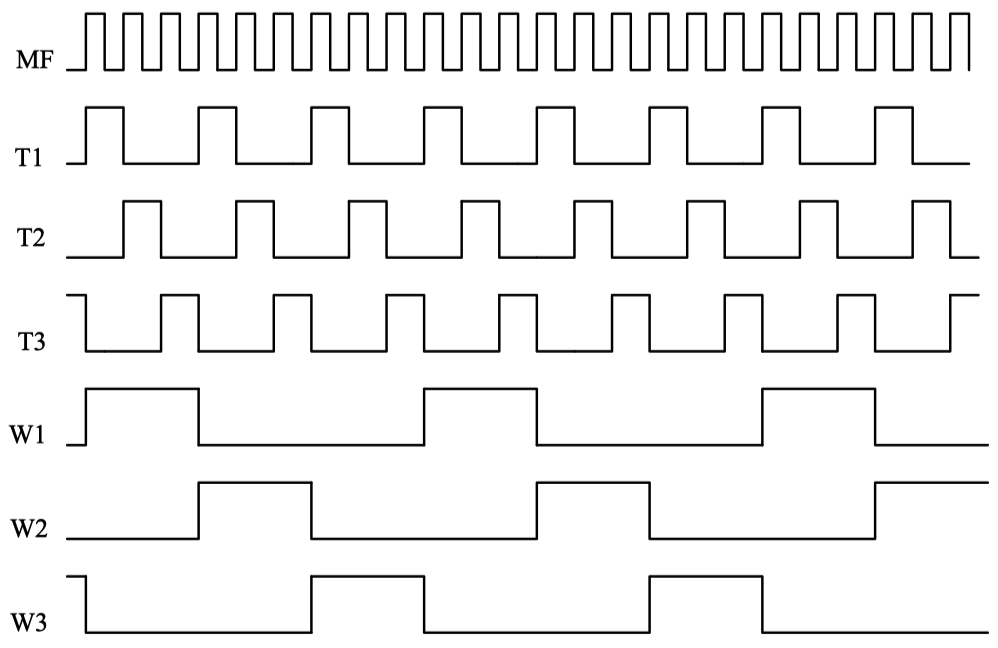
\includegraphics[width=0.7\linewidth]{./Images/clock.png}
    \caption{TEC-8模型计算机时序图\label{fig:clock}}
\end{figure}

\subsection{模型计算机组成}

TEC-8模型计算机的电路框图如\figref{fig:tec8model}。

\begin{figure}[htbp]
    \centering
    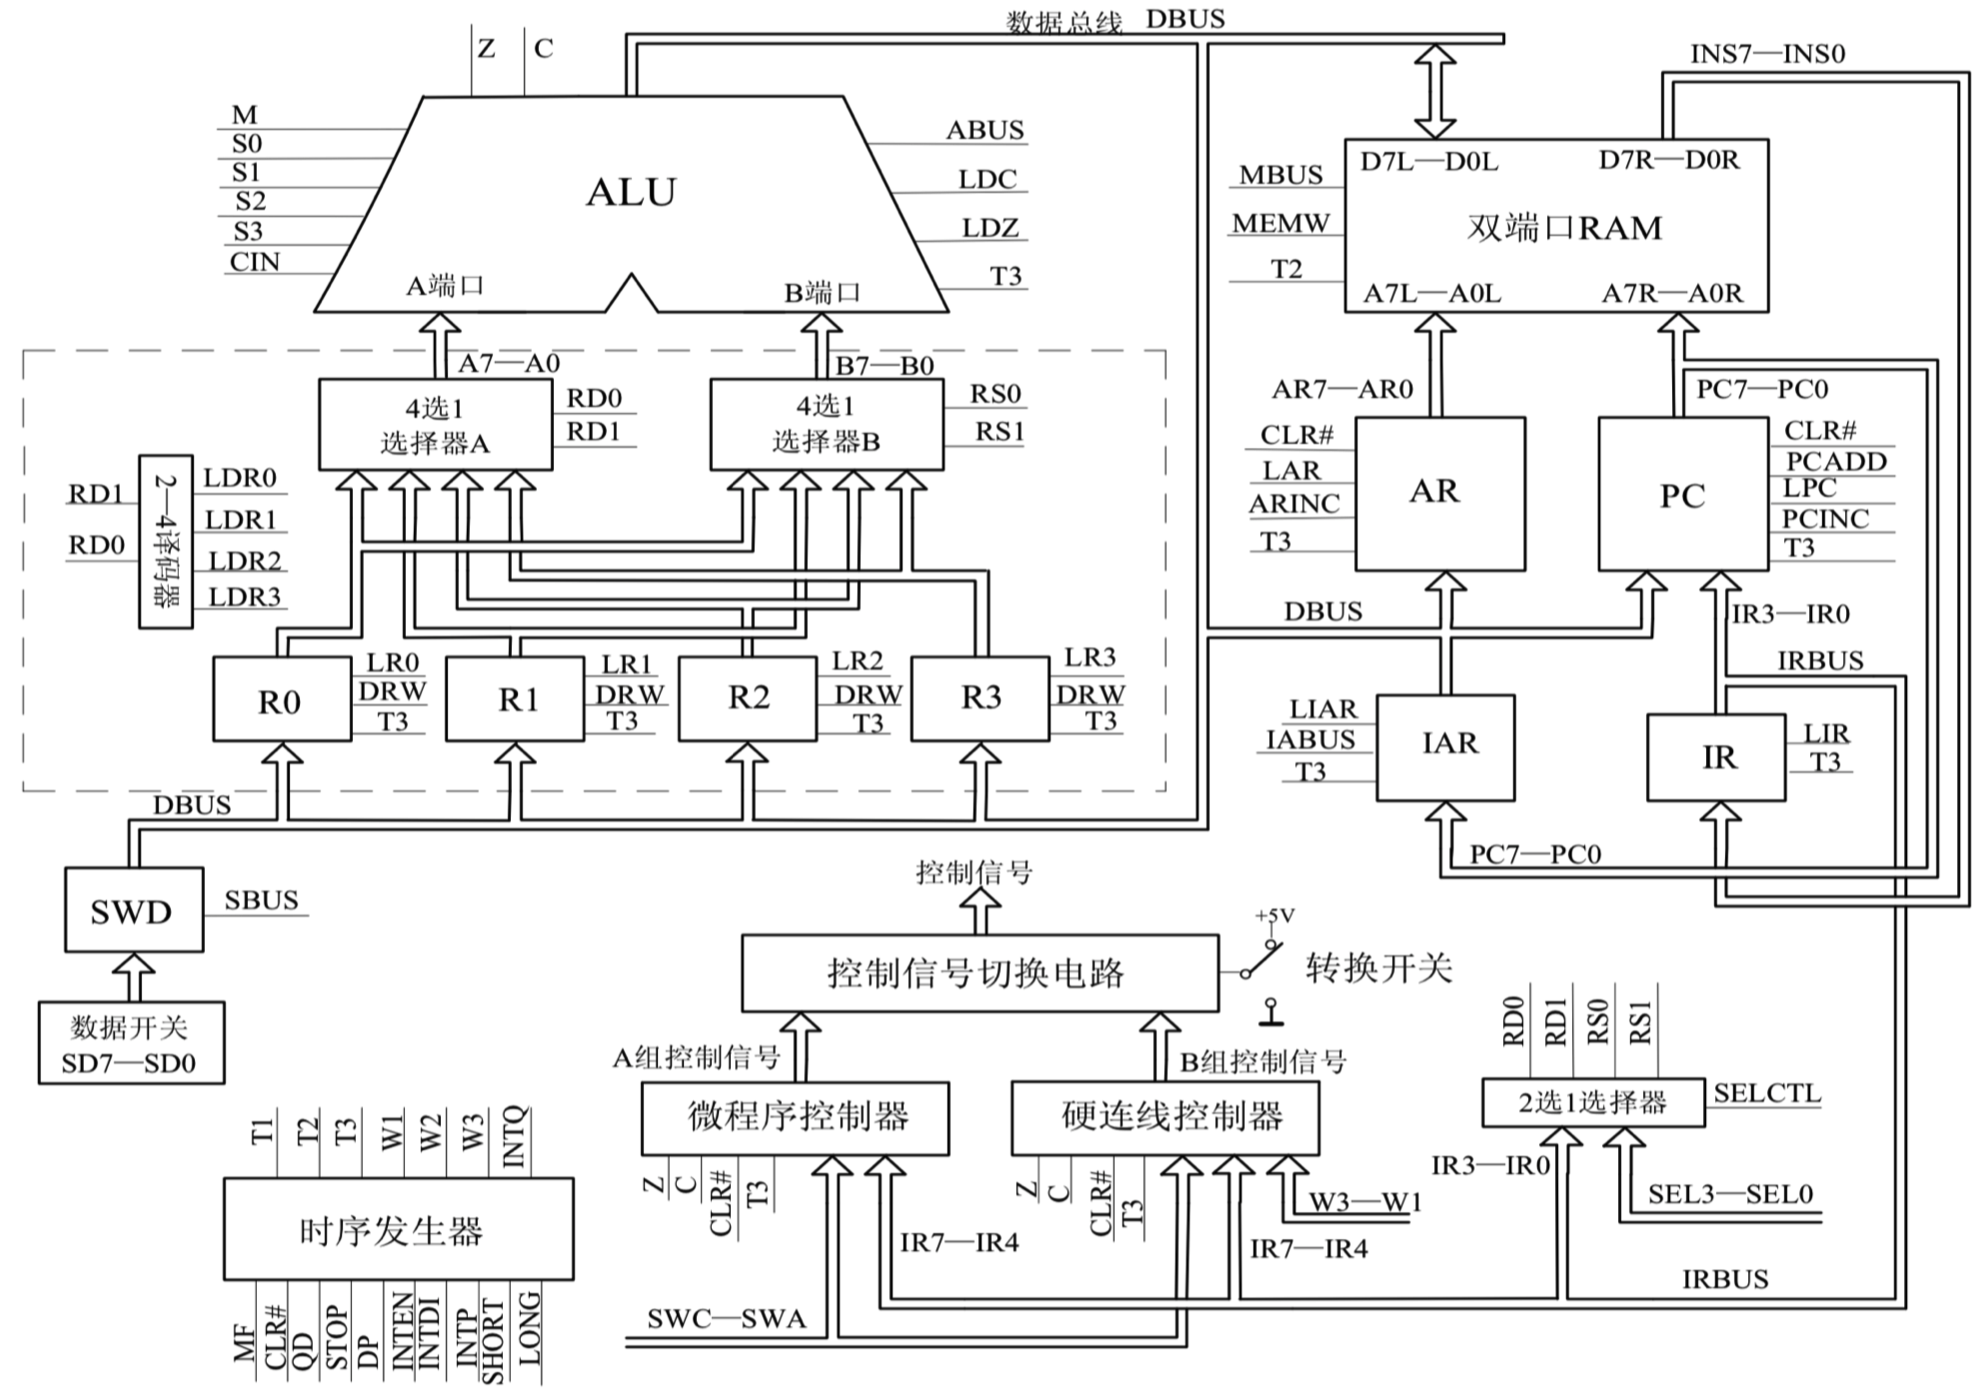
\includegraphics[width=\linewidth]{./Images/tec8model.png}
    \caption{TEC-8模型计算机框图\label{fig:tec8model}}
\end{figure}

\subsection{EPM7128引脚及信号说明}

硬连线控制器所需的信号的输出、输入信号的引脚号如\tabref{tab:signal}。

\begin{table}[!htbp]
    \centering
    \caption{作为硬连线控制器时的EPM7128引脚规定\label{tab:signal}}
    \begin{tabular}{|c|c|c|c|c|c|}
        \hline
        信号 & 方向 & 引脚号 & 信号 & 方向 & 引脚号 \\ \hline
        CLR\# & 输入 & 1 & MEMW & 输出 & 27 \\ \hline
        T3 & 输入 & 83 & STOP & 输出 & 28 \\ \hline
        SWA & 输入 & 4 & LIR & 输出 & 29 \\ \hline
        SWB & 输入 & 5 & LDZ & 输出 & 30 \\ \hline
        SWC & 输入 & 6 & LDC & 输出 & 31 \\ \hline
        IR4 & 输入 & 8 & CIN & 输出 & 33 \\ \hline
        IR5 & 输入 & 9 & S0 & 输出 & 34 \\ \hline
        IR6 & 输入 & 10 & S1 & 输出 & 35 \\ \hline
        IR7 & 输入 & 11 & S2 & 输出 & 36 \\ \hline
        W1 & 输入 & 12 & S3 & 输出 & 37 \\ \hline
        W2 & 输入 & 15 & M & 输出 & 39 \\ \hline
        W3 & 输入 & 16 & ABUS & 输出 & 40 \\ \hline
        C & 输入 & 2 & SBUS & 输出 & 41 \\ \hline
        Z & 输入 & 84 & MBUS & 输出 & 44 \\ \hline
        DRW & 输出 & 20 & SHORT & 输出 & 45 \\ \hline
        PCINC & 输出 & 21 & LONG & 输出 & 46 \\ \hline
        LPC & 输出 & 22 & SEL0 & 输出 & 48 \\ \hline
        LAR & 输出 & 25 & SEL1 & 输出 & 49 \\ \hline
        PCADD & 输出 & 18 & SEL2 & 输出 & 50 \\ \hline
        ARINC & 输出 & 24 & SEL3 & 输出 & 51 \\ \hline
        SELCTL & 输出 & 52 & & & \\ \hline
    \end{tabular}
\end{table}

各信号的说明如\tabref{tab:signaltab}。

\begin{table}[!htbp]
    \centering
    \caption{各信号的说明\label{tab:signaltab}}
    \resizebox{1.0\columnwidth}{!}{
    \begin{tabular}{|c|l|}
        \hline
        信号 & 说明 \\ \hline
        CLR\# & 复位。 \\ \hline
        T3 & 节拍脉冲信号 \\ \hline
        SWC、SWB、SWA & 操作模式选择。 \\ \hline
        IR7\textasciitilde IR4 & 指令寄存器的高四位。 \\ \hline
        W3\textasciitilde W1 & 节拍电位信号。 \\ \hline
        C & 进位标志。 \\ \hline
        Z & 结果为0标志。 \\ \hline
        DRW & \makecell[l]{=1时,在T3上升沿对RD1、RD0选中的寄存器进行写操作,将\\数据总线DBUS上的数D7\textasciitilde D0写入选定的寄存器。} \\ \hline
        PCINC & =1时,在T3的上升沿PC加1。 \\ \hline
        LPC	& \makecell[l]{=1时,在T3的上升沿,将数据总线DBUS上的D7\textasciitilde D0写入程序\\计数器PC。} \\ \hline
        LAR & \makecell[l]{=1时,在T3的上升沿,将数据总线DBUS上的D7\textasciitilde D0写入地址\\寄存器AR。} \\ \hline
        PCADD & =1时,将当前的PC值加上相对转移量,生成新的PC。 \\ \hline
        ARINC & =1时,在T3的上升沿,AR加1。 \\ \hline
        SETCTL & \makecell[l]{=1时,实验系统处于实验台状态。=0时,实验系统处于运行程序\\状态。} \\ \hline
        MEMW & \makecell[l]{=1时,在T2为1期间将数据总线DBUS上的D7\textasciitilde D0写入双端口\\RAM。写入的存储器单元由 AR7\textasciitilde AR0指定。} \\ \hline
        STOP & =1时,在T3结束后时序发生器停止输出节拍脉冲T1、T2、T3。 \\ \hline
        LIR & \makecell[l]{=1时,在T3的上升沿将从双端口RAM的右端口读出的指令\\INS7\textasciitilde INS0写入指令寄存器 IR。读出的存储器单元由PC7\textasciitilde PC0\\指定。} \\ \hline
        LDZ & \makecell[l]{=1时,如果运算结果为0,在T3的上升沿,将1写入到Z标志寄\\存器;如果运算结果不为0,将0保存到Z标志寄存器。} \\ \hline
        LDC & =1时,在T3的上升沿将运算得到的进位保存到C标志寄存器。 \\ \hline
        CIN & 低位74LS181的进位输入。 \\ \hline
        M & 运算模式:M=0为算术运算;M=1逻辑运算。 \\ \hline
        S3\textasciitilde S0 & 控制74LS181的运算类型。 \\ \hline
        ABUS & =1时,将运算结果送数据总线DBUS。 \\ \hline
        SBUS & =1时,数据开关SD7\textasciitilde SD0的数送数据总线DBUS。 \\ \hline
        MBUS & =1时,将双端口RAM的左端口数据送到数据总线DBUS。 \\ \hline
        SHORT & =1时,指示时序发生器只产生一个节拍电位。 \\ \hline
        LONG & =1时,指示时序发生器产生三个节拍电位。 \\ \hline
        SEL3\textasciitilde SEL2(RD1\textasciitilde RD0) & 选择送ALU的A端口的寄存器 \\ \hline
        SEL1\textasciitilde SEL0(RS1\textasciitilde RS0) & 选择送ALU的B端口的寄存器 \\ \hline
    \end{tabular}
    }
\end{table}

\subsection{硬连线控制器设计}

\subsubsection{硬连线控制器的基本原理}

每个微操作控制信号$S$是一系列输入量的逻辑函数,即用组合逻辑来实现:
$$
S = f(I_m, M_i, T_k, B_j)
$$
其中$I_m$是机器指令操作码译码器的输出信号,$M_i$是节拍电位信号,$T_k$是节拍脉冲信号,$B_j$是状态条件信号。
在TEC-8实验系统中,节拍脉冲信号$T_k$(T1\textasciitilde T3)已经直接输送给数据通路。
因为机器指令系统比较简单,省去操作码译码器,4位指令操作码IR4\textasciitilde IR7直接成为$I_m$的一部分;

由于TEC-8实验系统有控制台操作,控制台操作可以看作一些特殊的功能复杂的指令,因此SWC、SWB、SWA可以看作是$I_m$的另一部分。
$M_i$是时序发生器产生的节拍信号W1\textasciitilde W3;$B_j$包括ALU产生的进位信号C、结果为0信号Z等等。

\subsubsection{机器指令周期流程图设计}

设计微程序控制器使用流程图。设计硬连线控制器同样使用流程图。微程序控制器的控制信号以微指令周期为时间单位,硬连线控制器以节拍电位(CPU周期)为时间单位,两者在本质上是一样的,1个节拍电位时间和1条微指令时间都是从节拍脉冲T1的上升沿到T3的下降沿的一段时间。在微程序控制器流程图中,一个执行框代表一条微指令,在硬连线控制器流程图中,一个执行框代表一个节拍电位时间。

\subsubsection{执行一条机器指令的节拍电位数}

在TEC-8实验系统中,采用了可变节拍电位数来执行一条机器指令。大部分指令的执行只需2个节拍电位W1、W2,少数指令需要3个节拍电位W1、W2、W3。为了满足这种要求,在执行一条指令时除了产生完成指令功能所需的微操作控制信号外,对需要3个电位节拍的指令,还要求它在W2时产生一个信号LONG。信号LONG送往时序信号发生器,时序信号发生器接到信号LONG后产生节拍电位W3。

对于一些控制台操作,需要4个节拍电位才能完成规定的功能。为了满足这种情况,可以将控制台操作化成两条机器指令的节拍。为了区分写寄存器操作的2个不同阶段,可以用一个特殊的寄存器标志。

为了适应更为广泛的情况,TEC-8的时序信号发生器允许只产生一个节拍电位W1。当1条指令或者一个控制台在W1时,只要产生信号SHORT,该信号送往时序信号发生器,则时序信号发生器在W1后不产生节拍电位W2,下一个节拍仍是W1。

信号LONG和SHORT只对紧跟其后的第一个节拍电位的产生起作用。


\subsection{实验步骤}

\begin{enumerate}
    \item 设计一个硬连线控制器,和TEC-8模型计算机的数据通路结合在一起,构成一个完整的CPU,该CPU要求:
    \begin{enumerate}
        \item 能够完成控制台操作:启动程序运行、读存储器、写存储器、读寄存器和写寄存器。
        \item 能够执行\tabref{tab:command}中的指令,完成规定的指令功能。
    \end{enumerate}
    \item 在Quartus \uppercase\expandafter{\romannumeral2}下对硬连线控制器对设计方案进行编程和编译。
    \item 将编译后的硬连线控制器下载到TEC-8实验台上的ISP器件EPM7128中去,使EPM7128成为一个硬连线控制器。
    \item 根据指令系统,编写检测硬连线控制器正确性的测试程序,并用测试程序对硬布线控制器在单拍方式下进行调试,直到成功。
    \item 在调试成功的基础上,整理出设计文件。
\end{enumerate}

\begin{table}[!htbp]
    \centering
    \caption{指令系统\label{tab:command}}
    \begin{threeparttable}
    \begin{tabular}{|l|l|l|c|c|c|}
        \hline
        \multirow{2}{*}{名称} & \multirow{2}{*}{助记符} & \multirow{2}{*}{功能} & \multicolumn{3}{c|}{指令格式} \\ \cline{4-6}
        & & & IR7\textasciitilde IR4 & IR3\textasciitilde IR2 & IR1\textasciitilde IR0 \\ \hline
        空指令 & \mintinline{text}{NOP} & 无 & 0000 & XX\tnote{1} & XX \\ \hline
        加法 & \mintinline{text}{ADD Rd, Rs} & Rd $\leftarrow$ Rd\tnote{2} + Rs\tnote{3} & 0001 & Rd & Rs \\ \hline
        减法 & \mintinline{text}{SUB Rd, Rs} & Rd $\leftarrow$ Rd - Rs & 0010 & Rd & Rs \\ \hline
        逻辑与 & \mintinline{text}{AND Rd, Rs} & Rd $\leftarrow$ Rd $\wedge$ Rs & 0011 & Rd & Rs \\ \hline
        加1 & \mintinline{text}{INC Rd} & Rd $\leftarrow$ Rd + 1 & 0100 & Rd & XX \\ \hline
        取数 & \mintinline{text}{LD Rd, [Rs]} & Rd $\leftarrow$ [Rs] & 0101 & Rd & Rs \\ \hline
        存数 & \mintinline{text}{ST Rs, [Rd]} & Rs $\rightarrow$ [Rd] & 0110 & Rd & Rs \\ \hline
        C条件转移 & \mintinline{text}{JC addr} & \makecell[l]{如果C=1,\\则PC $\leftarrow$ @\tnote{4} + offset\tnote{5}} & 0111 & \multicolumn{2}{c|}{offset} \\ \hline
        Z条件转移 & \mintinline{text}{JZ addr} & \makecell[l]{如果Z=1,\\则PC $\leftarrow$ @ + offset} & 1000 & \multicolumn{2}{c|}{offset} \\ \hline
        无条件转移 & \mintinline{text}{JMP [Rd]} & PC $\leftarrow$ Rd & 1001 & Rd & XX \\ \hline
        输出 & \mintinline{text}{OUT [Rs]} & DBUS $\leftarrow$ Rs & 1010 & XX & Rs \\ \hline
        逻辑或 & \mintinline{text}{OR Rd, Rs} & Rd $\leftarrow$ Rd $\vee$ Rs & 1011 & Rd & Rs \\ \hline
        比较 & \mintinline{text}{CMP Rd, Rs} & Rd - Rs & 1100 & Rd & Rs \\ \hline
        移动值 & \mintinline{text}{MOV Rd, Rs} & Rd $\leftarrow$ Rs & 1101 & Rd & Rs \\ \hline
        停机 & \mintinline{text}{STOP} & 暂停运行 & 1110 & XX & XX \\ \hline
    \end{tabular}
    \begin{tablenotes}
    \footnotesize
        \item[1] XX代表随意值。
        \item[2] Rs代表源寄存器号。
        \item[3] Rd代表目的寄存器号。
        \item[4] @代表当前PC的值。
        \item[5] offset是一个4位的补码有符号数。
    \end{tablenotes}
    \end{threeparttable}
\end{table}

\section{设计详解}

\subsection{基础功能}

该CPU需要完成的功能可以分为两类,一类完成控制台操作,即根据SWC、SWB、SWA的不同值来读写寄存器、存储器或启动程序运行;另一类执行机器指令,即根据IR0\textasciitilde IR3的值来执行不同的指令。分析机器指令流程图可得,第一类操作都可以分成两个机器周期完成,第二类操作的大部分指令都在可以在两个机器周期完成(少数需要三个机器周期)第一个周期为取指周期,第二个周期为执行周期。下面详细分析每个功能如何实现。

\subsubsection{写寄存器}

当SWC SWB SWA=100的时候,进入写寄存器状态,一共需要四个机器周期,分别写寄存器R0、R1、R2、R3,根据标志位ST0的值将它分为两个阶段,每个阶段两个节拍,当ST0=0时,执行第一个阶段,当ST0=1时,执行第二个阶段。

写每个寄存器时,都需要使SBUS=1,DRW=1,而不同点主要在于SEL0\textasciitilde SEL3的值,SEL3\textasciitilde SEL2指定当前写入的寄存器,SEL1\textasciitilde SEL0指定上次写入的寄存器即当前读出的寄存器。例如,第一个W1时SEL3\textasciitilde SEL2=00,SEL1\textasciitilde SEL0=11,表示写入寄存器R0,第一个W2时SEL3\textasciitilde SEL2=01,SEL1\textasciitilde SEL0=00,表示写入寄存器R1,并读取R0的值(指示灯B7\textasciitilde B0),以此类推。同时为了辅助ST0的改变,设置SST0标志位,在第一个W2节拍时,使 SST0=1,ST0检测到W2\&SST0=1时,会由0变为1,标志着进入到第二个W1、W2。

在写寄存器的第四拍将ST0重新设置为0,如果再进行下一拍则重新从R0开始写入。

\subsubsection{读寄存器}

当SWC SWB SWA=011的时候,进入读寄存器状态,一共需要两个机器周期,W1读寄存器R0、R1,W2读寄存器R2、R3。

根据SEL3\textasciitilde SEL0的值选择不同的寄存器,SEL3\textasciitilde SEL2决定A端口指示的寄存器,SEL1\textasciitilde SEL0决定B端口指示的寄存器,W1时SEL3\textasciitilde SEL2=00,SEL1\textasciitilde SEL0=01,ALU的A端口(指示灯A7\textasciitilde A0)指示寄存器R0的值,ALU的B端口(指示灯B7\textasciitilde B0)指示寄存器R1的值。之后的W2节拍类似,改变SEL的值读出R2、R3寄存器的值。

\subsubsection{写存储器}

当SWC SWB SWA=001的时候,进入写存储器状态,根据标志位ST0的值将它分为两个阶段,每个阶段只有一个机器周期。第一个阶段指定首地址,第二个阶段不断循环,地址自加后依次写入存储单元。

第一个阶段时ST0=0,SBUS=1,LAR=1,将数据开关的值送入地址寄存器 AR,指定了写存储器的首地址,然后将SST0置为1,表示下一拍将进入ST0=1的阶段。第二个阶段时ST0=1,MEMW=1,把当前数据总线上的值存入指定存储单元,然后ARINC=1,将AR加1,在下一个节拍中向下一个存储单元写入值,不断循环直到CLR。

\subsubsection{读存储器}

当SWC SWB SWA=010的时候,进入读存储器状态,与写存储器类似,同样根据标志位ST0的值将它分为两个阶段,每个阶段只有一个机器周期。第一个阶段指定首地址,第二个阶段不断循环,地址自加后依次读存储单元。

第一个阶段时ST0=0,SBUS=1,LAR=1,将数据开关的值送入地址寄存器AR,指定了读存储器的首地址,然后将SST0置为1,表示下一拍将进入ST0=1的阶段。第二个阶段时ST0=1,MBUS=1,把存储单元的值读到数据总线上,然后ARINC=1,将AR加1,在下一个节拍中读取下一个存储单元的值,不断循环直到CLR。

\subsubsection{执行指令}

当SWC SWB SWA=000的时候,进入执行程序状态,第一个机器周期取指令,第二个机器周期进入执行指令阶段,之后在每条指令结束时再取指令,再执行,不断循环直到STOP。

第一个阶段时,PCINC=1,LIR=1,取出当前的指令到IR,PC自加1,指向下一条指令的地址,第二个阶段时根据IR7\textasciitilde IR4的值进入不同的分支执行指令,指令执行结束的时候再取下一条指令。

\subsubsection{扩展指令}

在原指令的基础上,我们新增了五条扩展指令,如\tabref{tab:extendedcommand}。

\begin{table}[!htbp]
    \centering
    \caption{扩展指令\label{tab:extendedcommand}}
    \begin{tabular}{|l|l|l|c|c|c|}
        \hline
        \multirow{2}{*}{名称} & \multirow{2}{*}{助记符} & \multirow{2}{*}{功能} & \multicolumn{3}{c|}{指令格式} \\ \cline{4-6}
        & & & IR7\textasciitilde IR4 & IR3\textasciitilde IR2 & IR1\textasciitilde IR0 \\ \hline
        空指令 & \mintinline{text}{NOP} & 无 & 0000 & XX & XX \\ \hline
        输出 & \mintinline{text}{OUT [Rs]} & DBUS $\leftarrow$ Rs & 1010 & XX & Rs \\ \hline
        逻辑或 & \mintinline{text}{OR Rd, Rs} & Rd $\leftarrow$ Rd $\vee$ Rs & 1011 & Rd & Rs \\ \hline
        比较 & \mintinline{text}{CMP Rd, Rs} & Rd - Rs & 1100 & Rd & Rs \\ \hline
        移动值 & \mintinline{text}{MOV Rd, Rs} & Rd $\leftarrow$ Rs & 1101 & Rd & Rs \\ \hline
    \end{tabular}
\end{table}

这些指令的流程图如\figref{fig:extended-ins}所示。

\begin{figure}[htbp]
    \centering
    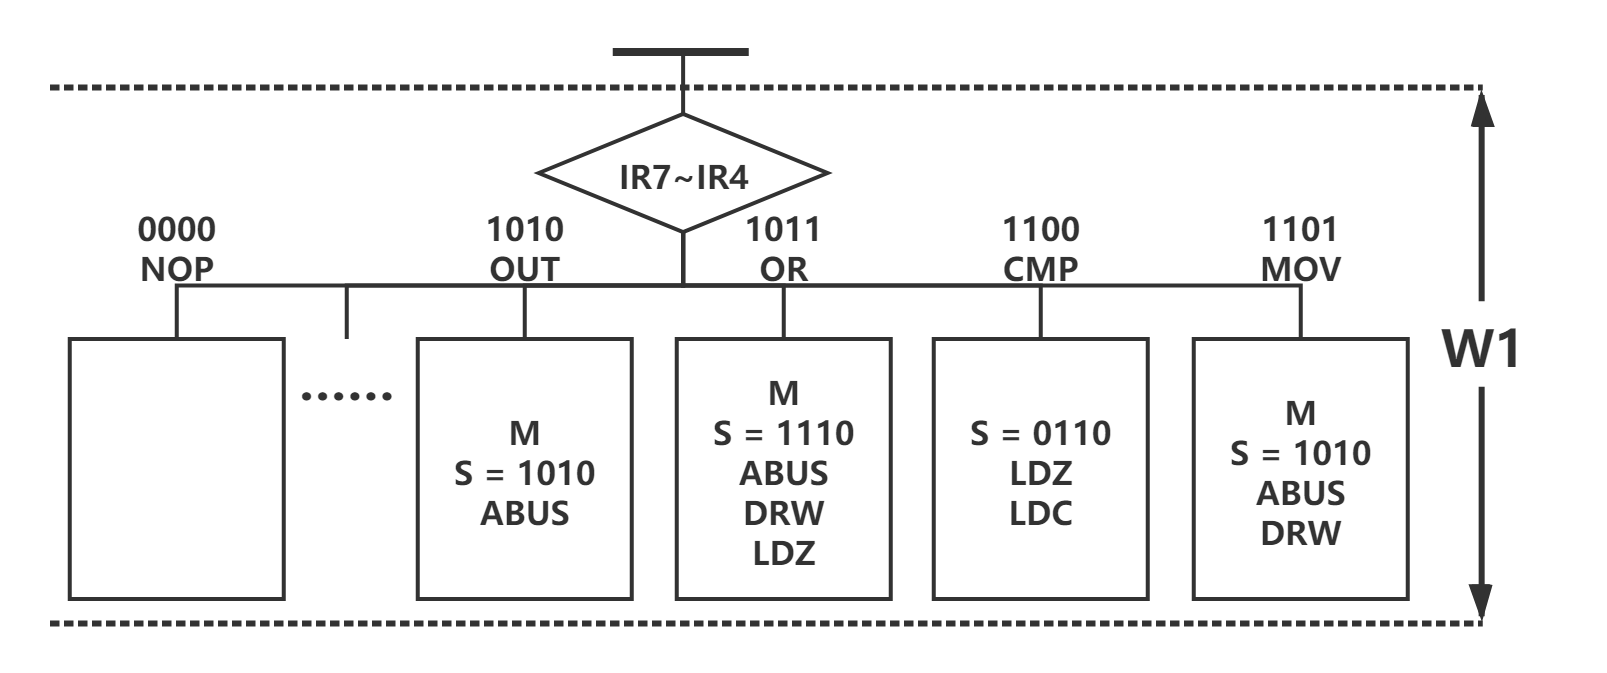
\includegraphics[width=0.8\linewidth]{./Images/extended-ins.png}
    \caption{扩展指令流程图\label{fig:extended-ins}}
\end{figure}

\subsubsection{用户指定PC功能}

在执行指令的基础上扩展后可实现用户指定PC功能。指定PC的原理与写寄存器的原理类似,即在程序开始执行前要将数据开关的值打到PC里,作为程序的首地址。通过标志位ST0将它分为两个阶段。第一个阶段指定程序存放的首地址,第二个阶段是取指令、执行指令。

第一个阶段ST0=0,SBUS=1,LPC=1,将数据开关上的值存到PC里,实现了指定程序首地址,并且将ST0置为1;第二阶段即是正常的取指令阶段,ST0=1,PCINC=1,LIR=1,开始不断取指令并执行指令。

此功能的流程图如\figref{fig:nopipe-pc}所示。

\begin{figure}[htbp]
    \centering
    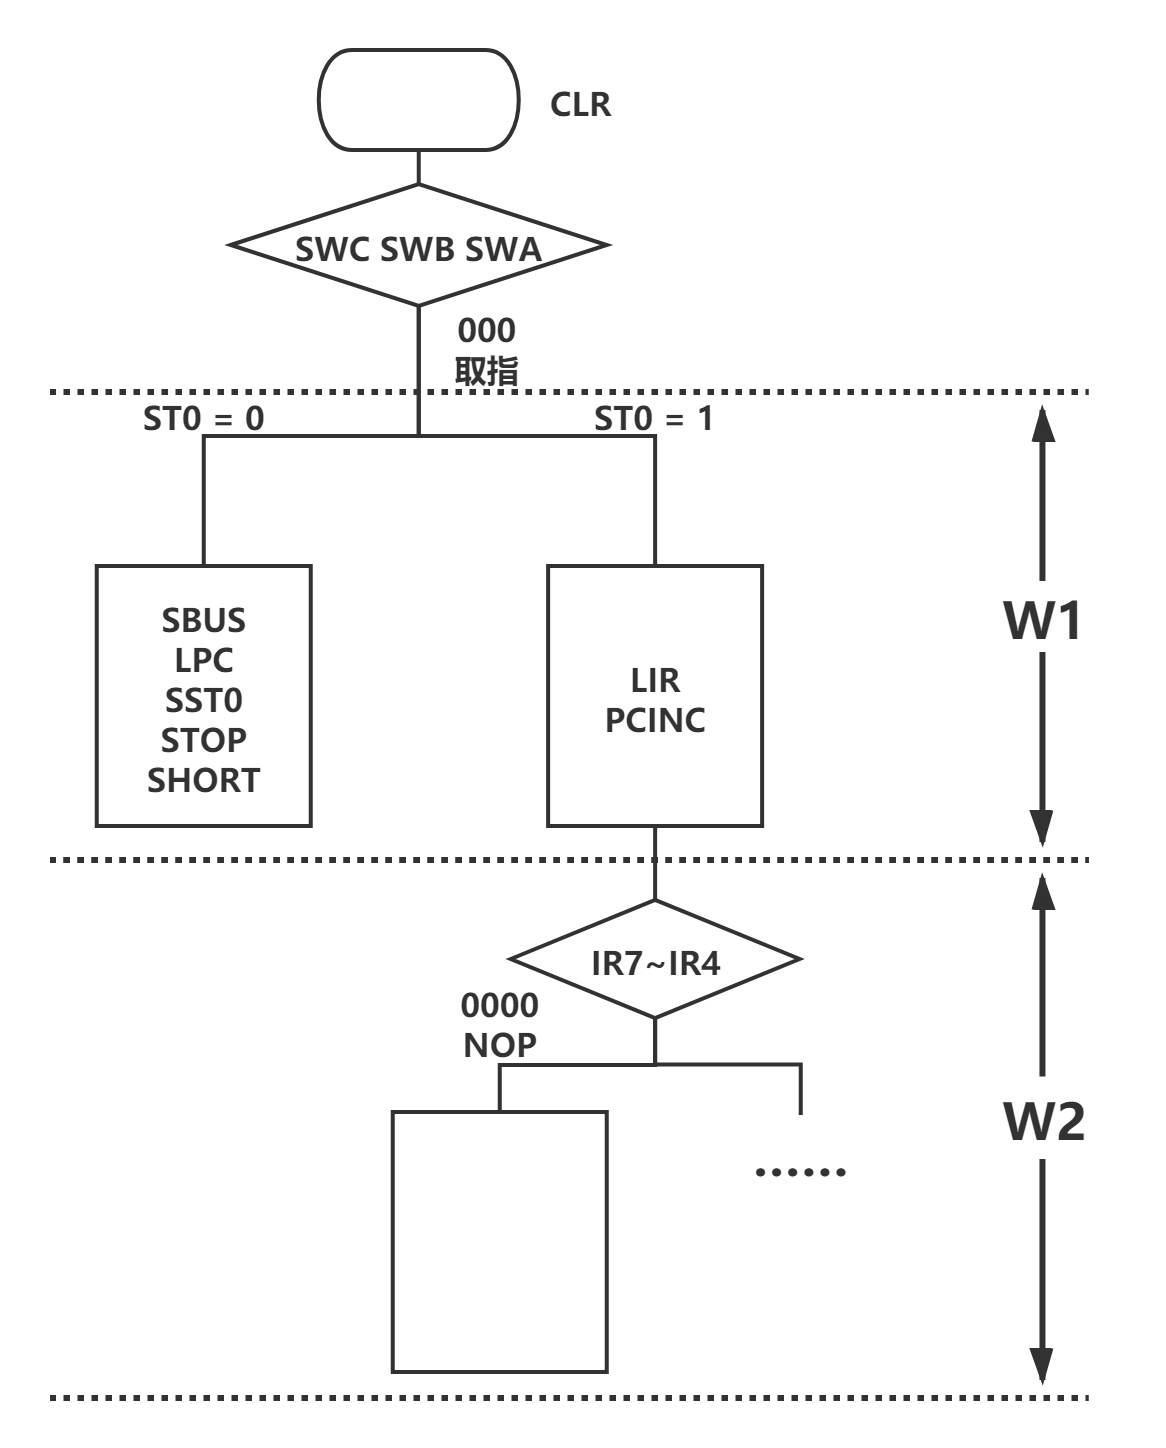
\includegraphics[width=0.5\linewidth]{./Images/nopipe-pc.png}
    \caption{用户指定PC功能流程图\label{fig:nopipe-pc}}
\end{figure}

\subsubsection{指令译码表}


在机器指令周期流程图的基础上,我们就可以根据流程图来编写译码表,译码表的首行列出了所有的指令信号,首列列出了所有的控制信号,每一个格子表示在什么指令和什么条件下需要发出什么信号。横着看每一行,表示需要发出该控制信号的所有情况;竖着看每一列,表示该条指令在W1,W2节拍下需要发出的所有控制信号。针对流水与非流水情况,分别设计了两张译码表。相比非流水情况下,流水情况下的译码表要更加复杂,每一拍需要发出的控制信号更多。

指令中用到的运算器的功能如\tabref{tab:alutab}所示,指令译码表如\figref{fig:code-table}所示。

\begin{figure}[htbp]
    \centering
    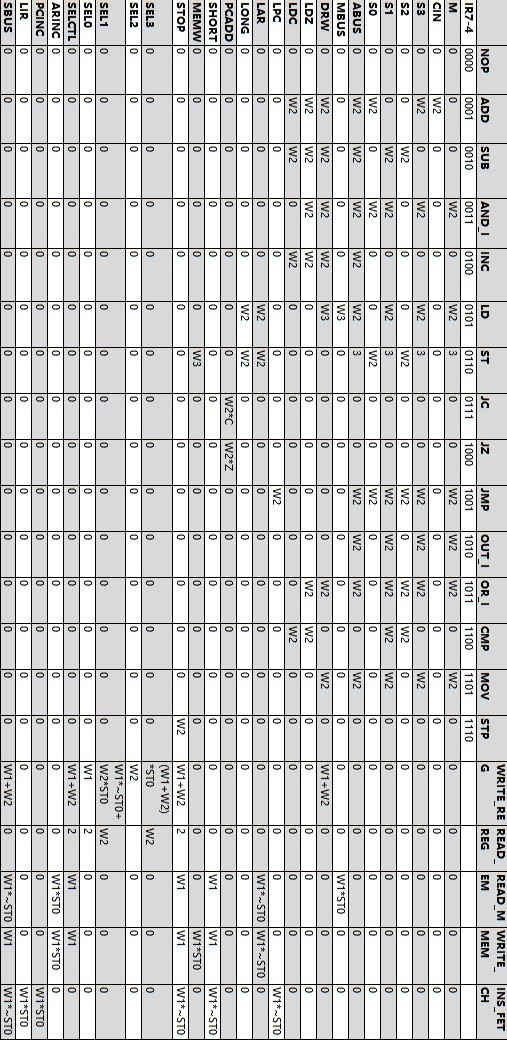
\includegraphics[width=0.73\linewidth]{./Images/code-table.jpg}
    \caption{指令译码表\label{fig:code-table}}
\end{figure}

\begin{table}[!htbp]
    \centering
    \caption{ALU逻辑/算术功能表\label{tab:alutab}}
    \begin{tabular}{|c|l|l|}
        \hline
        S (ALU工作方式选择输入) & M = 1 (逻辑运算)  & M = 0 (算术运算) \\ \hline
        $0000$ & $\overline{A}$ & $A+1$ \\ \hline
        $0110$ & $\overline{A \oplus B}$ & $A-B-1$ \\ \hline
        $1001$ & $\overline{A \oplus B}$ & $A+B$ \\ \hline
        $1010$ & $B$ & $(A\vee\overline B)+A\wedge B$ \\ \hline
        $1011$ & $A\wedge B$ & $A\wedge B-1$ \\ \hline
        $1110$ & $A\vee B$ & $(A\vee\overline B)+A$ \\ \hline
        $1111$ & $A$ & $A-1$ \\ \hline
    \end{tabular}
\end{table}

\subsubsection{程序实现}

硬布线控制器的程序实现有两种风格,我们分别称之为数据流描述和行为描述,数据流描述是基于如\figref{fig:code-table}的译码表的描述,即采用逻辑表达式实现所有信号。行为描述是基于指令流程图,这种实现方式不需要写出译码表,根据流程图的判断条件写出程序即可,这两种描述方式的代码框架如\coderef{code:dataflow}和\coderef{code:behave}。

\begin{code}
\caption{数据流描述\label{code:dataflow}}
\begin{minted}{VHDL}
-- 操作模式
    WRITE_REG <= '1' when SW = "100" else '0';
    READ_REG <= '1' when SW = "011" else '0';
    INS_FETCH <= '1' when SW = "000" else '0';
    READ_MEM <= '1' when SW = "010" else '0';
    WRITE_MEM <= '1' when SW = "001" else '0';
    
-- 操作码
    ADD <= '1' when IR = "0001" and INS_FETCH = '1' and ST0 = '1' else '0';
    SUB <= '1' when IR = "0010" and INS_FETCH = '1' and ST0 = '1' else '0';
    
    OUT_I <= '1' when IR = "1010" and INS_FETCH = '1' and ST0 = '1' else '0';
    OR_I <= '1' when IR = "1011" and INS_FETCH = '1' and ST0 = '1' else '0';
    CMP <= '1' when IR = "1100" and INS_FETCH = '1' and ST0 = '1' else '0';
    MOV <= '1' when IR = "1101" and INS_FETCH = '1' and ST0 = '1' else '0;
    
-- ST0 状态
    process(CLR, T3, W)
    begin
        if (CLR = '0') then
            ST0 <= '0';
        elsif (T3'event and T3 = '0') then
            if (ST0 = '0' and ((WRITE_REG = '1' and W(2) = '1') or (READ_MEM = '1' and W(1) = '1') or (WRITE_MEM = '1' and W(1) = '1') or (INS_FETCH = '1' and W(1) = '1'))) then
                ST0 <= '1';
            elsif (ST0 = '1' and (WRITE_REG = '1' and W(2) = '1')) then
                ST0 <= '0';
            end if;
        end if;
    end process;

-- 控制信号合成
    SBUS <= ((WRITE_REG or (READ_MEM and not ST0) or WRITE_MEM or (INS_FETCH and not ST0)) and W(1)) or (WRITE_REG and W(2));
    DRW <= (WRITE_REG and (W(1) or W(2))) or ((ADD or SUB or AND_I or INC or OR_I or MOV) and W(2)) or (LD and W(3));

\end{minted}
\end{code}

\begin{code}
\caption{行为描述\label{code:behave}}
\begin{minted}{VHDL}
    process (SW, IR,  W(1),  W(2),  W(3), T3 ,CLR, C, Z, ST0, SST0) 
    begin
-- 初始化控制信号
-- ST0 状态
        if (clr = '0') then
            ST0 <= '0';
        else
            if (T3'event and T3 = '0') and SST0 = '1' then
                ST0 <= '1';
            end if;

            case SW is
-- --------------------------------------------------------------------
                -- WRITE_MEM
                when "001" =>
-- --------------------------------------------------------------------
                -- READ_MEM
                when "010" =>
-- --------------------------------------------------------------------
                -- READ_REG
                when "011" =>
-- --------------------------------------------------------------------
                -- WRITE_REG
                when "100" =>
-- --------------------------------------------------------------------
                -- INS_FETCH
                when "000" =>
--------------------------------------------------------------------
                    -- 用户置入PC的值指定程序初始位置
                    if ST0 = '0' then
                        LPC <=  W(1); -- 用户置入PC的值指定程序初始位置
                        SBUS <=  W(1);
                        SST0 <=  W(1);
                        SHORT <=  W(1);
                        STOP <=  W(1);
                        SELCTL <=  W(1);
--------------------------------------------------------------------
                    -- 执行程序
                    else -- ST0='1'
                        LIR <=  W(1);
                        PCINC <=  W(1);
                        case IR is
                            when "0001" => -- ADD
                                S <=  W(2) & '0' & '0' &  W(2);
                                CIN <=  W(2);
                                ABUS <=  W(2);
                                DRW <=  W(2);
                                LDZ <=  W(2);
                                LDC <=  W(2);
                            when "0010" => -- SUB
                                S <= '0' &  W(2) &  W(2) & '0';
                                ABUS <=  W(2);
                                DRW <=  W(2);
                                LDZ <=  W(2);
                                LDC <=  W(2);
                            when others => null; -- IR
                        end case; -- IR
                    end if; -- ST0='1'
                when others => null;--SW="000"
            end case; -- SW
        end if; -- clr='1'
    end process;


\end{minted}
\end{code}




\subsection{流水线}

指令周期中包含两个子过程,取指令和执行指令。\figref{fig:nopipe-tsgraph}为非流水计算机的时空图,对于非流水计算机来说,上一条指令的两个子过程全部执行完毕之后才能开始下一条指令。因此,每隔2个机器时钟周期才有一个输出结果。

\figref{fig:pipe-tsgraph}为流水计算机的时空图,对于流水计算机来说,上一条指令与下一条指令的子过程在时间上可以重叠执行。因此,当流水线满载时,每一个时钟周期就可以输出一个结果。

对于需要两个节拍电位的指令,如LD和ST,则在其第二拍(W2)时取下一条指令,时空图如\figref{fig:pipe-ld-tsgraph}所示。

\begin{figure}[htbp]
    \centering
    \subfigure[非流水时空图\label{fig:nopipe-tsgraph}]{
        \begin{minipage}[t]{0.41\linewidth}
            \centering
            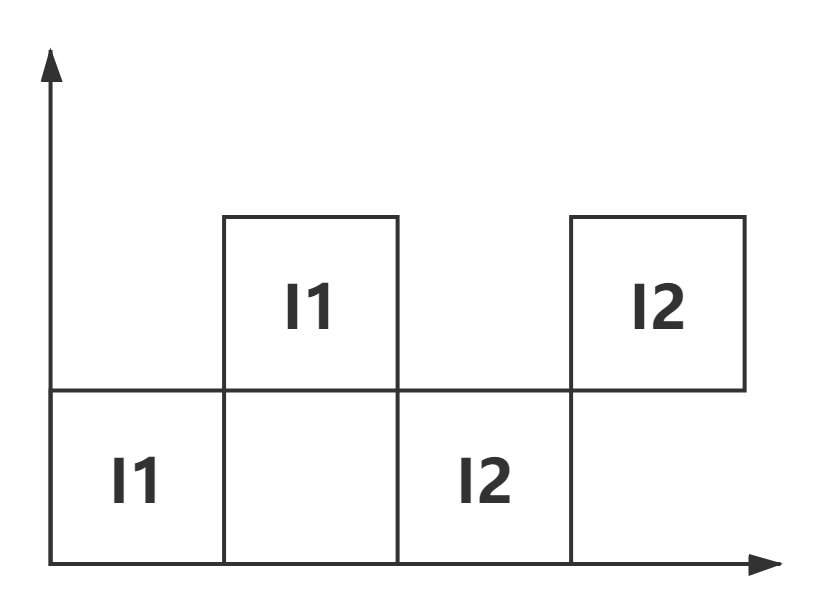
\includegraphics[width=\linewidth]{./Images/nopipe-tsgraph.png}
        \end{minipage}
    }
    \subfigure[流水时空图\label{fig:pipe-tsgraph}]{
        \begin{minipage}[t]{0.5\linewidth}
            \centering
            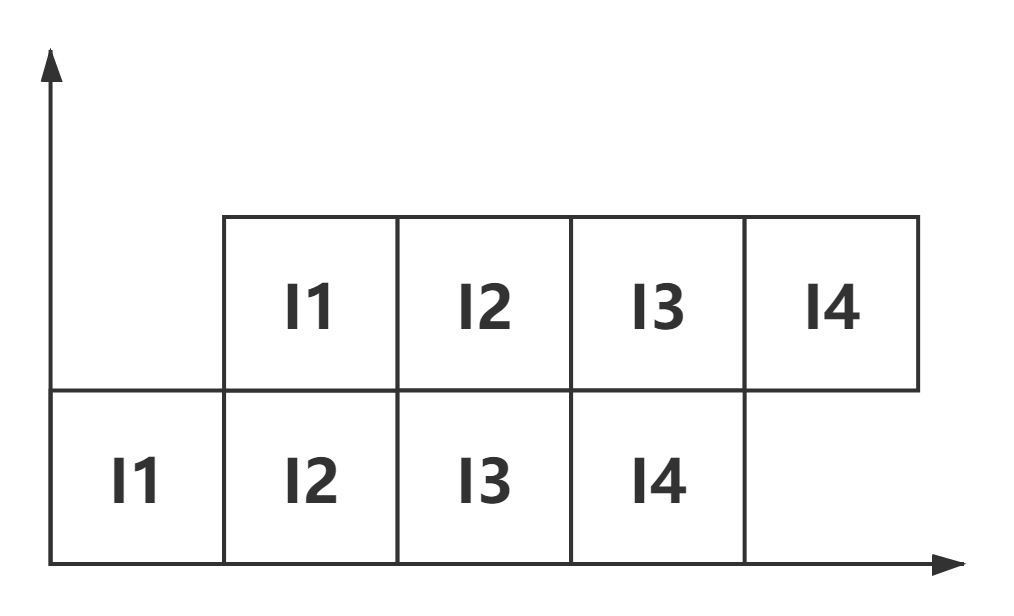
\includegraphics[width=\linewidth]{./Images/pipe-tsgraph.png}
        \end{minipage}
    }
    
    \subfigure[两拍指令的流水时空图\label{fig:pipe-ld-tsgraph}]{
        \begin{minipage}[t]{0.5\linewidth}
            \centering
            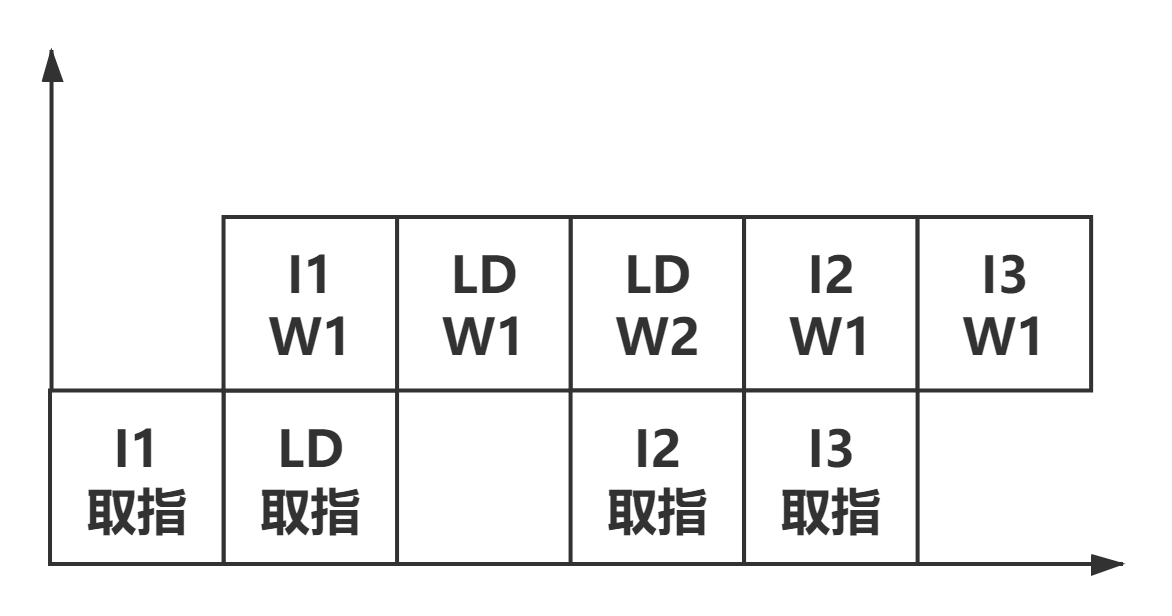
\includegraphics[width=\textwidth]{./Images/pipe-ld-tsgraph.png}
        \end{minipage}
    }
    \caption{时空图}
\end{figure}

流水线的具体实现方式就是将上一条指令的执行指令和下一条指令的取指令部分合并到一个节拍电位中进行,其流程图如\figref{fig:pipe-flow}所示。

相应地,扩展指令的流程也要做类似的改动。由于第一条指令之前没有取指令阶段,所以在用户指定PC后加一个节拍电位,用于进行第一个指令的取指令,其流程图如\figref{fig:pipe-pc}所示。

\begin{figure}[htbp]
    \centering
    \subfigure[无扩展指令\label{fig:pipe-flow}]{
        \begin{minipage}[t]{0.95\linewidth}
            \centering
            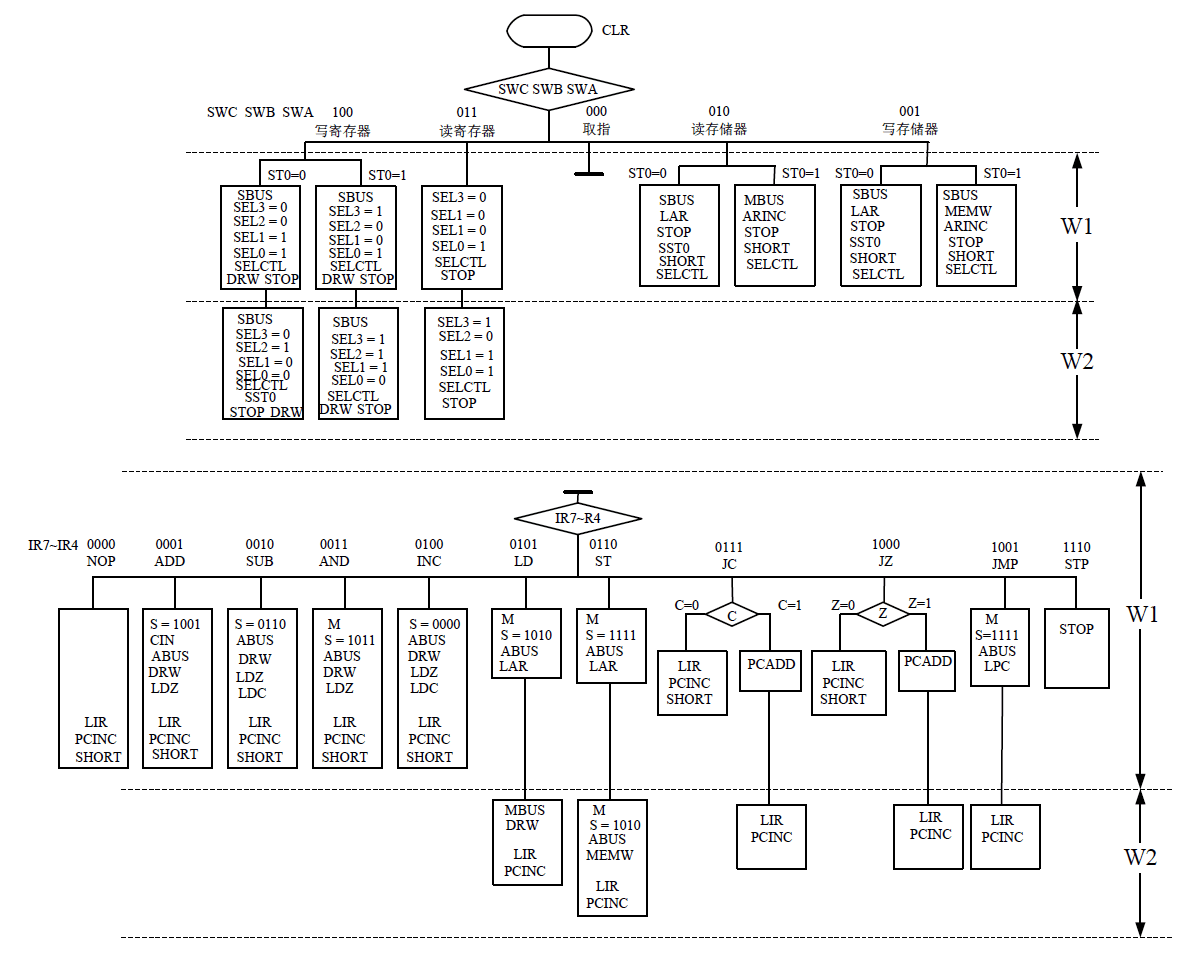
\includegraphics[width=\linewidth]{./Images/pipe-flow.png}
        \end{minipage}
    }
    
    \subfigure[用户指定PC功能\label{fig:pipe-pc}]{
        \begin{minipage}[t]{0.5\linewidth}
            \centering
            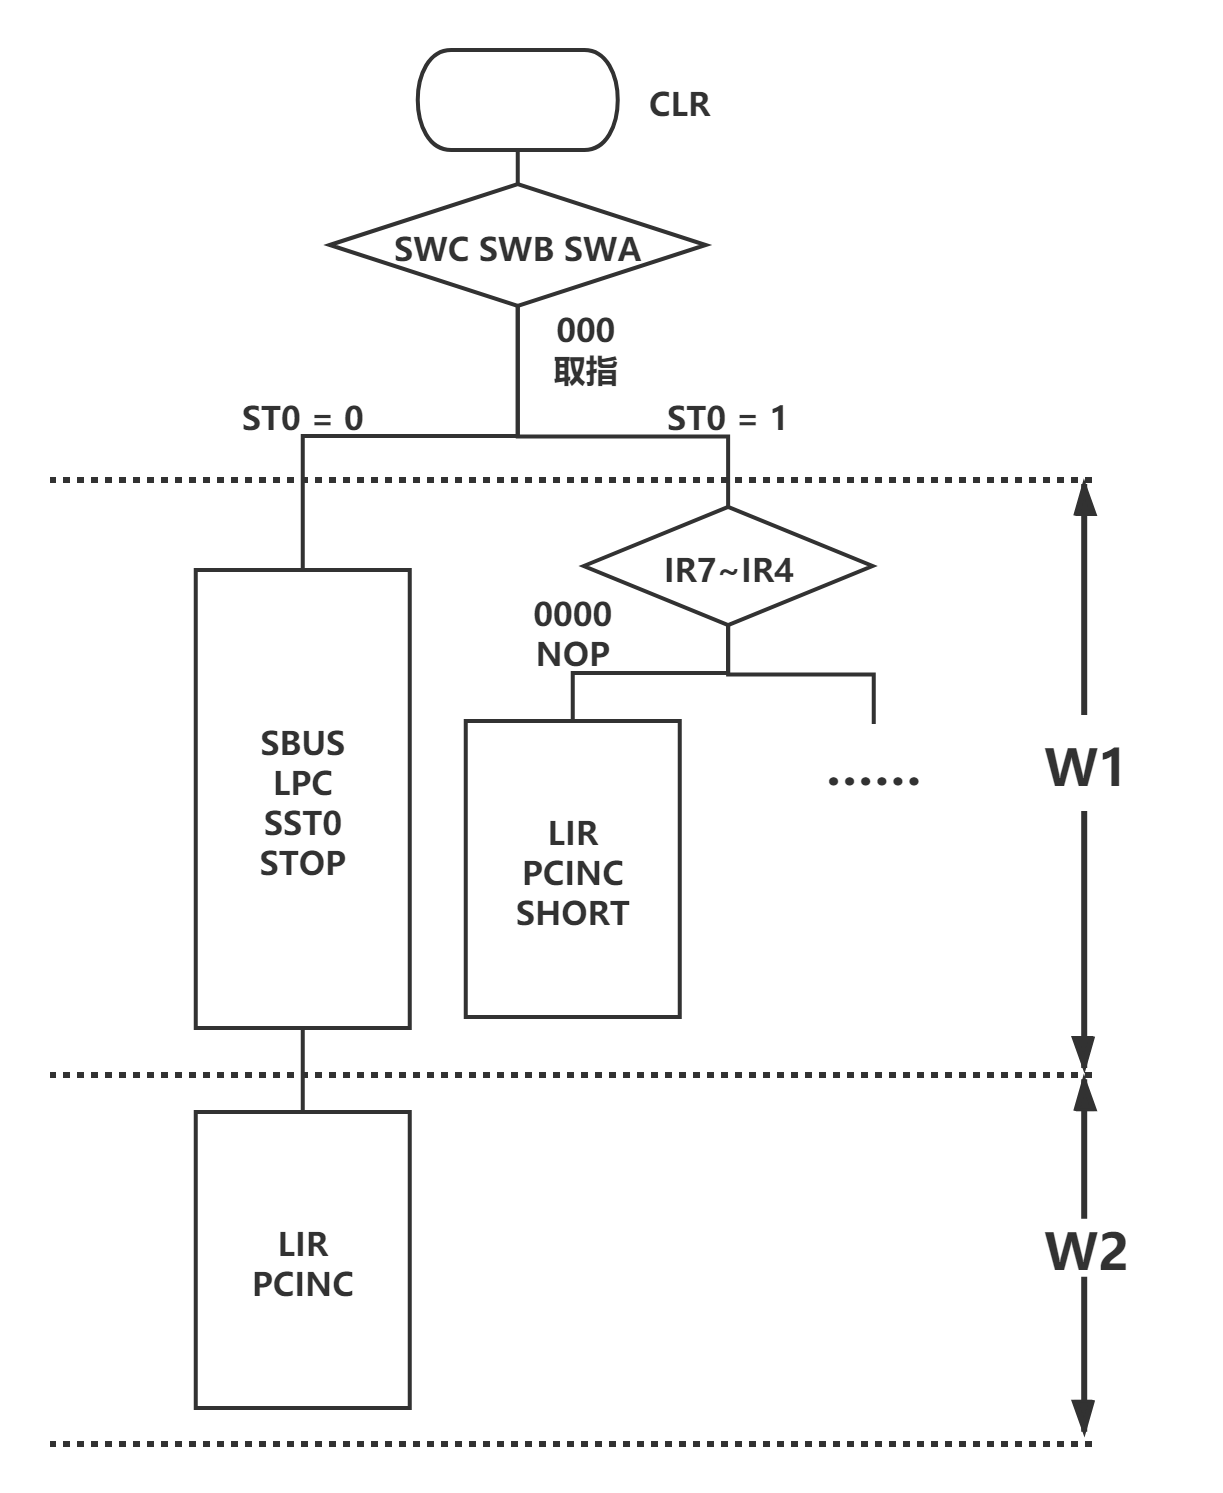
\includegraphics[width=\textwidth]{./Images/pipe-pc.png}
        \end{minipage}
    }
    \caption{流水线流程图}
\end{figure}

指令译码表如\figref{fig:pipe-code-table}所示。其中,$S_3\sim S_0$参考\tabref{tab:alutab}。

\begin{figure}[htbp]
    \centering
    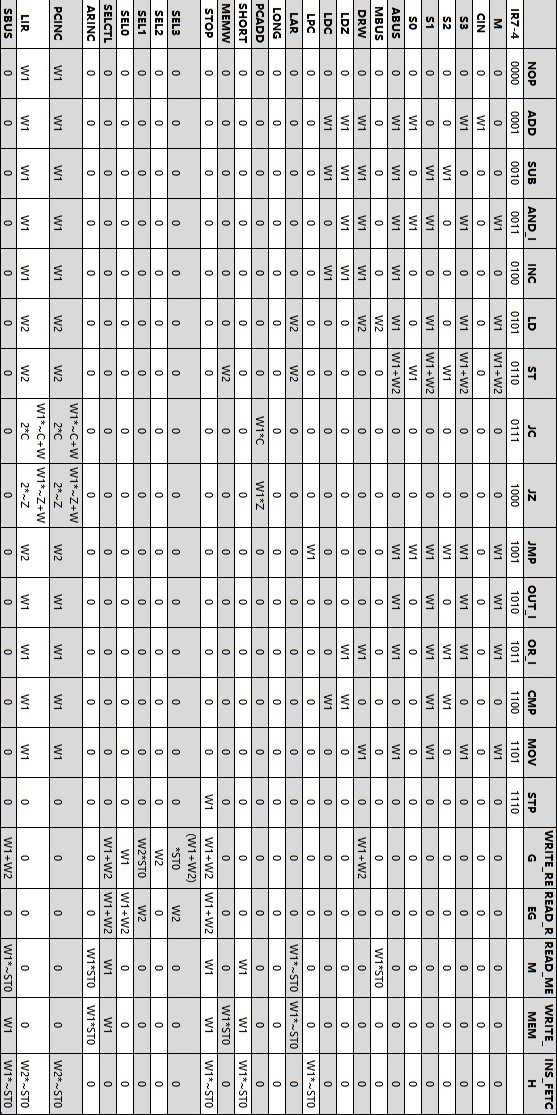
\includegraphics[width=0.75\linewidth]{./Images/pipe-code-table.jpg}
    \caption{流水线指令译码表\label{fig:pipe-code-table}}
\end{figure}

\subsection{中断}

由于EPM7128芯片中没有接入LIAR和IABUS管脚,因此我们无法控制IAR寄存器,也就无法读出和暂存PC的值,意味着我们中断之后无法返回断点,这给我们实现中断带来了很大的困难。经过老师的提示,我们采用R3寄存器同步PC的值,在中断返回时将R3的值赋给PC,以达到回到断点的目的。

\subsubsection{对指令集的改动}

我们首先对原有的指令集进行如下改动:

\paragraph{指令中只能访问R0\textasciitilde R2寄存器} R3寄存器用于同步PC的值,所以其他指令不能访问该寄存器。

\paragraph{不支持JZ和JC指令} 这两个指令的低四位表示偏移量,我们无法直接读出IR3\textasciitilde IR0,因此无法实现R3与PC同步变化。理论上可以通过双端口存储器的左端口读出指令,再通过逻辑与运算分离出低四位,再给R3加上这四位得到结果,但是这一系列操作可能需要6个以上的节拍电位,过于复杂,由于时间限制而未予实现。

\paragraph{JMP指令改动} JMP指令除了要将寄存器中的值赋给PC之外,还要赋给R3,因此需要对指令格式和指令流程进行改动。具体而言,JMP指令的指令格式如\tabref{tab:jmpcommand}所示。之前程序中的JMP指令仍然按照原有格式。

\paragraph{新增IRET指令} 此指令用于从中断服务程序中返回,它的职能包括开中断、将寄存器R3的值赋给PC,指令格式如\tabref{tab:jmpcommand}。

\begin{table}[!htbp]
    \centering
    \caption{指令系统\label{tab:jmpcommand}}
    \begin{tabular}{|l|l|l|c|c|c|}
        \hline
        \multirow{2}{*}{名称} & \multirow{2}{*}{助记符} & \multirow{2}{*}{功能} & \multicolumn{3}{c|}{指令格式} \\ \cline{4-6}
        & & & IR7\textasciitilde IR4 & IR3\textasciitilde IR2 & IR1\textasciitilde IR0 \\ \hline
        无条件转移 & \mintinline{text}{JMP [Rd]} & PC $\leftarrow$ Rd & 1001 & 11 & Rd \\ \hline
        中断返回 & \mintinline{text}{IRET} & PC $\leftarrow$ R3 & 1111 & XX & XX \\ \hline
    \end{tabular}
\end{table}

\subsubsection{新增的信号和标志}

此外,新增了一个输入信号PULSE,从61引脚输入,表示中断脉冲信号。

程序中新增了一些标志,如\tabref{tab:signalexp}所示。

\begin{table}[!htbp]
    \centering
    \caption{各标志位的说明\label{tab:signalexp}}
    \begin{tabular}{|c|l|}
        \hline
        标志 & 说明 \\ \hline
        INT & 中断标志。 \\ \hline
        EN\_INT & 中断允许标志。 \\ \hline
        ST1 & 中断周期标志。 \\ \hline
        INTDI & =1时,置允许中断标志为0,禁止TEC-8模型计算机响应中断请求。 \\ \hline
        INTEN & =1时,置允许中断标志为1,允许TEC-8模型计算机响应中断请求。 \\ \hline
    \end{tabular}
\end{table}

\subsubsection{中断流程}

中断部分的流程图如\figref{fig:interrupt}所示。

\begin{figure}[htbp]
    \centering
    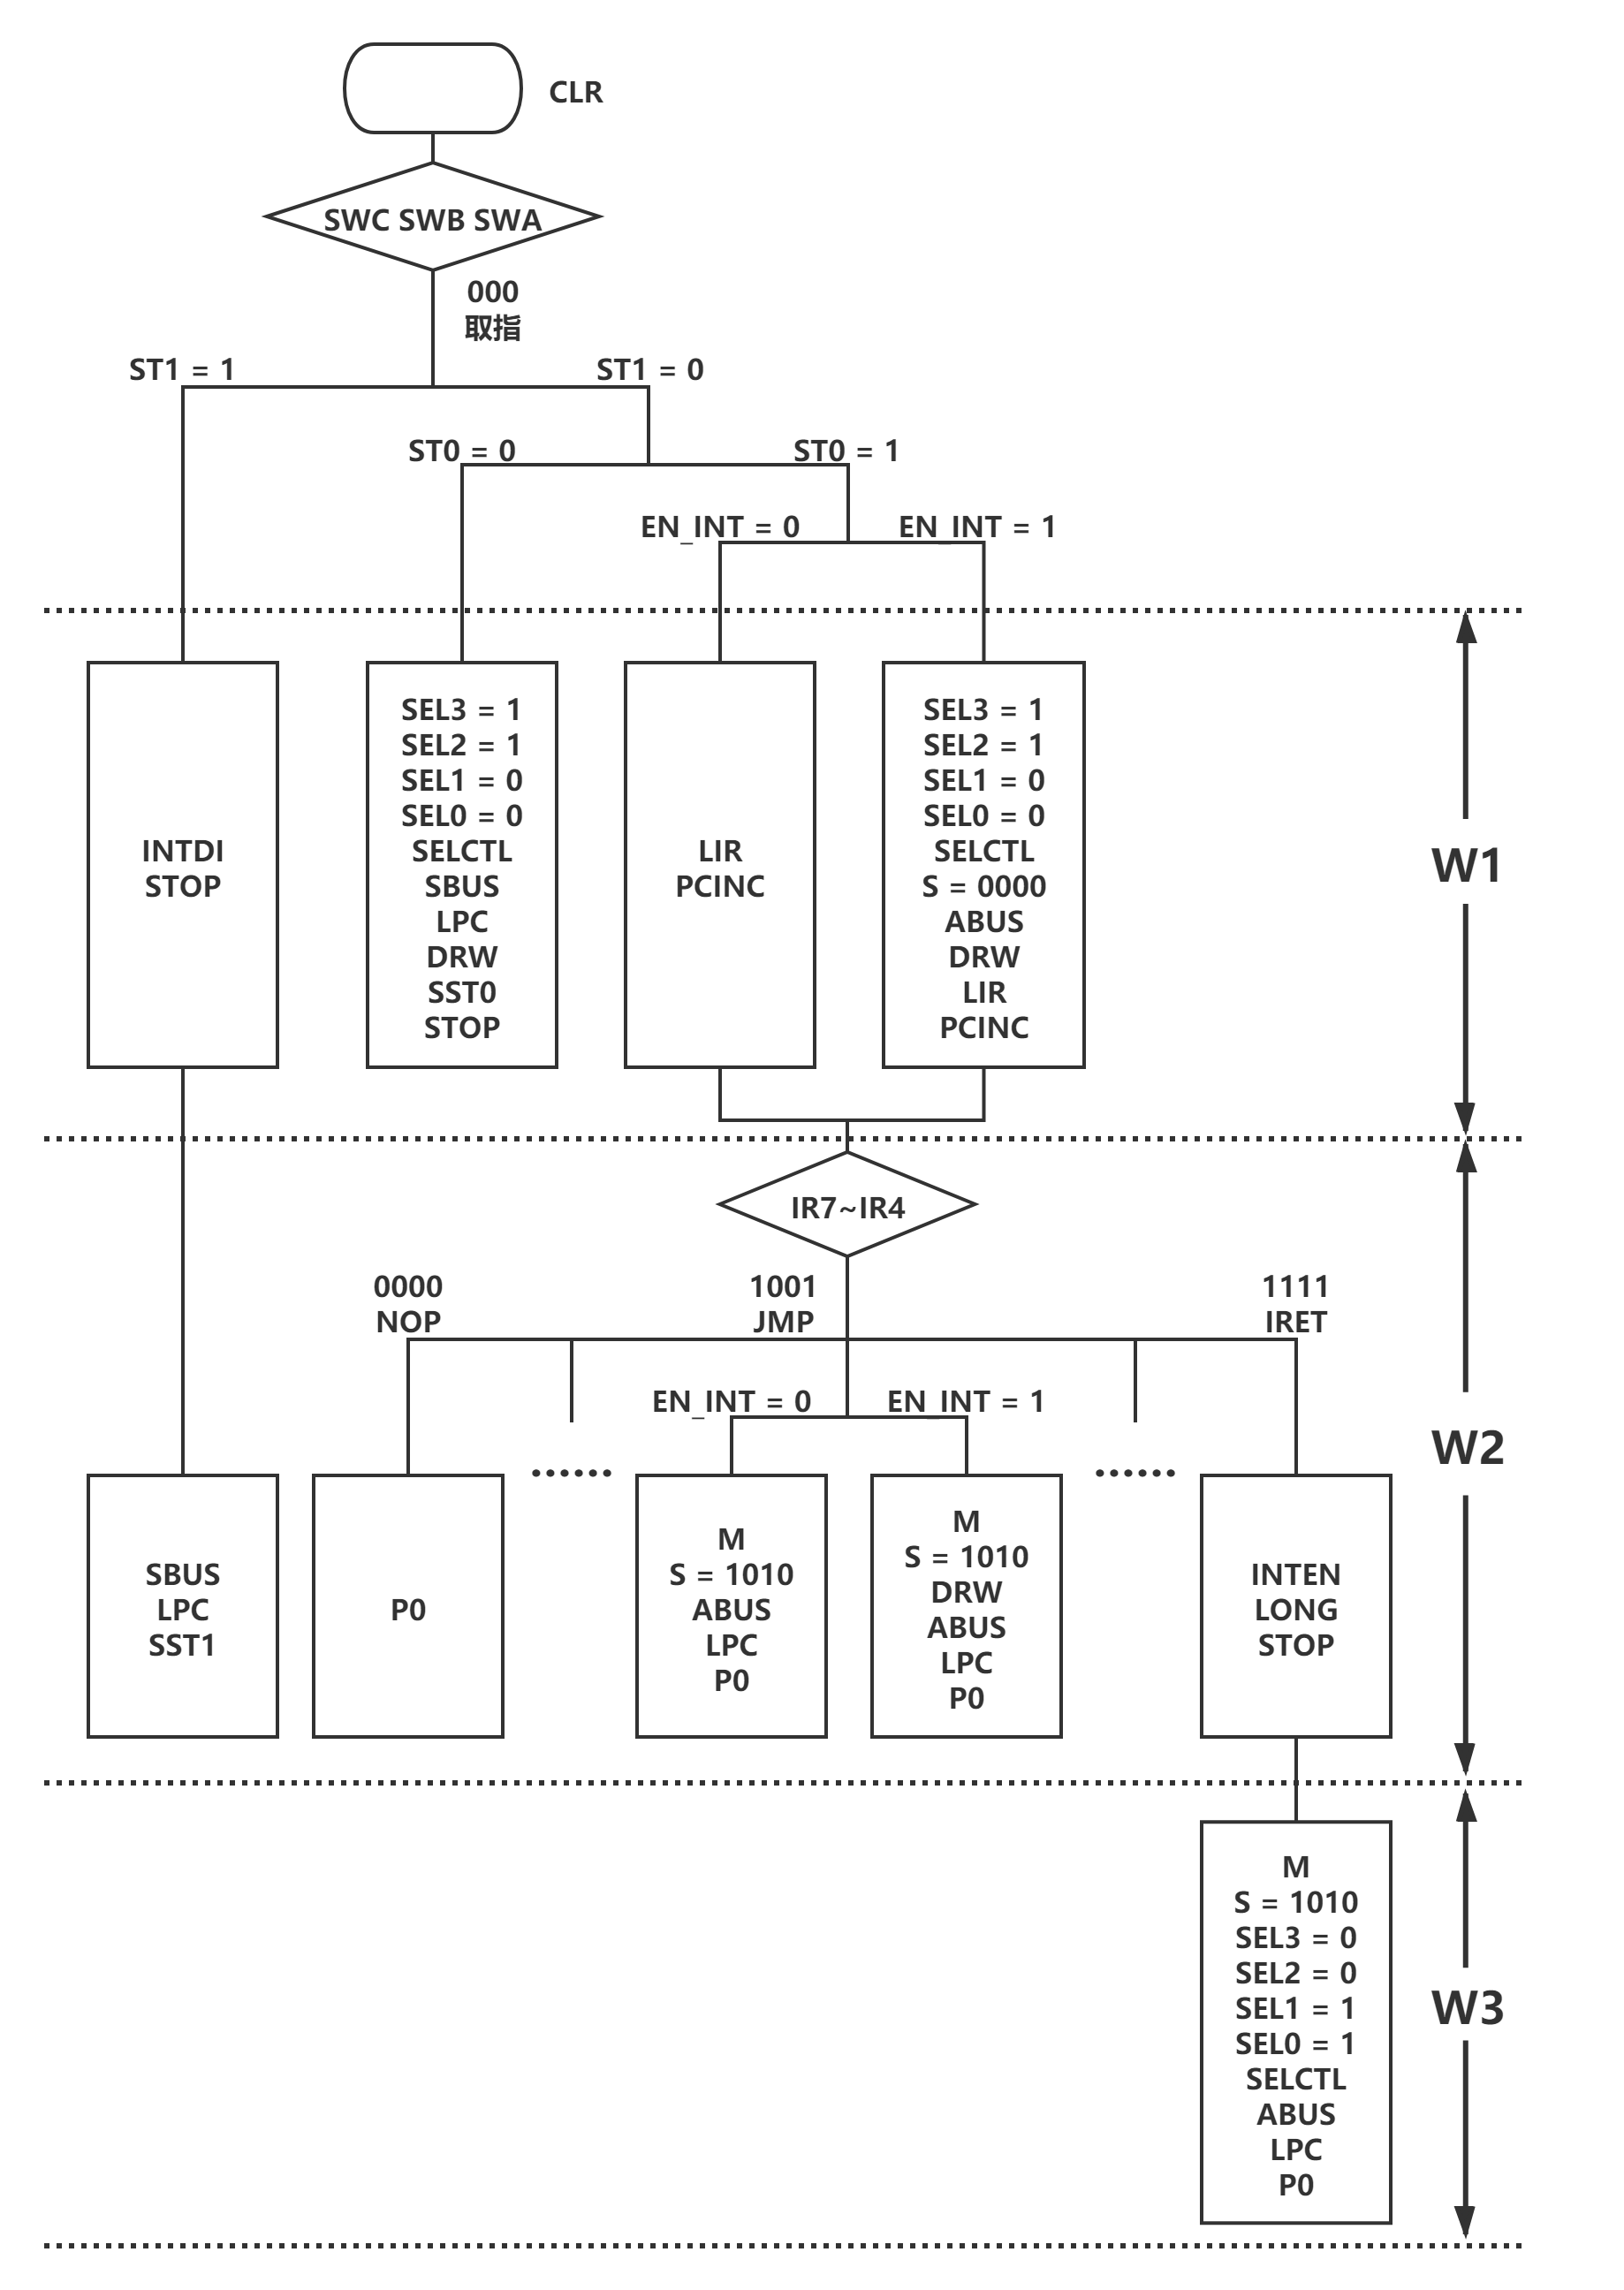
\includegraphics[width=0.8\linewidth]{./Images/interrupt.png}
    \caption{中断流程图\label{fig:interrupt}}
\end{figure}

\paragraph{R3与PC同步}

为了使R3与PC同步,需要对程序的PCINC和JMP指令做一些改动。

当取指令时,同时利用ALU的运算使R3自增1;当执行JMP时,由于预先规定IR3\textasciitilde IR2为11,此时设置DRW为1即可将另一寄存器的值同时写入PC和R3。

\paragraph{中断周期}

默认状态下(即按下CLR后),中断允许标志EN\_INT为1,中断标志INT为0。即默认开中断,没有手动开中断的指令。

在每个时钟周期的上升沿,根据INTDI和INTEN来设置中断允许标志;当按下PULSE时,根据中断允许标志来设置INT的值;在每条指令执行的最后一个节拍电位的T3上升沿,如果此时INT为1,则设置ST1为1(在流程图中写作P0),表示之后进入中断周期。

中断周期中,首先关中断,并且暂停程序等待写入PC的值,之后在W2的T3上升沿将ST1置为0,表示中断周期结束,之后进入中断处理程序。

\paragraph{中断处理程序}

中断处理程序与主程序差异不大,只是R3和PC不需要同步,因此PCINC和JMP指令不对R3做更改。由于我们只实现了单级中断,所以执行处理程序时仍然处于关中断状态,因此可以根据是否开中断来判断是否正在执行中断处理程序。

中断处理程序必须以IRET指令结束,表示回到主程序。IRET指令的W2拍开中断,W3拍将R3的值赋给PC,以达到恢复断点的目的。

由于W2拍已经开中断,所以在W3拍仍然可以开始中断,将在IRET指令执行结束之后再次进入中断周期。

\section{调试总结}

\subsection{测试结果}

\subsubsection{测试集1}

此测试集主要用于测试\mintinline{text}{LD}、\mintinline{text}{INC}、\mintinline{text}{SUB}、\mintinline{text}{ST}、\mintinline{text}{ADD}、\mintinline{text}{JC}、\mintinline{text}{AND}、\mintinline{text}{OUT}、\mintinline{text}{STP}指令,指令如\tabref{tab:base_test_1}所示,初始状态下寄存器R2 = 12H,R3 = 0FH,存储器[0FH] = 85H,[10H] = 23H,[11H] = EFH。

\begin{table}[!htbp]
    \centering
    \caption{测试集1\label{tab:base_test_1}}
    \begin{tabular}{|l|l|l|l|l|}
        \hline 
        地址 & 指令 & 机器码 & 功能 & 结果 \\ \hline 
        00H & \mintinline{text}{LD R0, [R3]} & 0101 0011 & R0 $\leftarrow$ [R3] & R0 $\leftarrow$ 85H \\ \hline 
        01H & \mintinline{text}{INC R3} & 0100 1100 & R3 $\leftarrow$ R3 + 1 & R3 $\leftarrow$ 10H \\ \hline 
        02H & \mintinline{text}{LD R1, [R3]} & 0101 0111 & R1 $\leftarrow$ [R3] & R1 $\leftarrow$ 23H \\ \hline 
        03H & \mintinline{text}{SUB R0, R1} & 0010 0001 & R0 $\leftarrow$ R0 - R1 & R0 $\leftarrow$ 62H \\ \hline 
        04H & \mintinline{text}{JZ 0BH} & 1000 0110 & \makecell[l]{如果Z=1,\\则PC $\leftarrow$ @ + 06H} & \makecell[l]{Z=0,\\不跳转} \\ \hline 
        05H & \mintinline{text}{ST R0, [R2]} & 0110 1000 & R0 $\rightarrow$ [R2] & 62H $\rightarrow$ [12H]  \\ \hline 
        06H & \mintinline{text}{INC R3} & 0100 1100 & R3 $\leftarrow$ R3 + 1 & R3 $\leftarrow$ 11H \\ \hline 
        07H & \mintinline{text}{LD R0, [R3]} & 0101 0011 & R0 $\leftarrow$ [R3]  & R0 $\leftarrow$ EFH \\ \hline 
        08H & \mintinline{text}{ADD R0, R1} & 0001 0001 & R0 $\leftarrow$ R0 + R1 & R0 $\leftarrow$ 12H \\ \hline 
        09H & \mintinline{text}{JC 0CH} & 0111 0010 & \makecell[l]{如果C=1,\\ 则PC $\leftarrow$ @ + 02H} & \makecell[l]{C=1,\\PC $\leftarrow$ 0CH} \\ \hline 
        0AH & \mintinline{text}{INC R2} & 0100 1000 &  &  \\ \hline 
        0BH & \mintinline{text}{ST R2, [R2]} & 0110 1010 &  &  \\ \hline 
        0CH & \mintinline{text}{AND R0, R1} & 0011 0001 & R0 $\leftarrow$ R0 $\wedge$ R1 & R0 $\leftarrow$ 02H \\ \hline 
        0DH & \mintinline{text}{OUT R2} & 1010 0010 & DBUS $\leftarrow$ R2 & DBUS $\leftarrow$ 12H \\ \hline 
        0EH & \mintinline{text}{STP} & 1110 0000 & 暂停运行 &  \\ \hline
    \end{tabular}
\end{table}

\subsubsection{测试集2}

此测试集主要用于测试\mintinline{text}{JC}指令,指令如\tabref{tab:base_test_2}所示,初始状态下寄存器R2 = 12H,R3 = 0FH,存储器[0FH] = 23H,[10H] = 23H,[11H] = EFH。

\begin{table}[!htbp]
    \centering
    \caption{测试集2\label{tab:base_test_2}}
    \begin{tabular}{|l|l|l|l|l|}
        \hline 
        地址 & 指令 & 机器码  &  功能 & 结果 \\ \hline 
        00H & \mintinline{text}{LD R0, [R3]} & 0101 0011  &  R0 $\leftarrow$ [R3] & R0 $\leftarrow$ 23H \\ \hline 
        01H & \mintinline{text}{INC R3} & 0100 1100  &  R3 $\leftarrow$ R3 + 1 & R3 $\leftarrow$ 10H \\ \hline 
        02H & \mintinline{text}{LD R1, [R3]} & 0101 0111  &  R1 $\leftarrow$ [R3]  & R1 $\leftarrow$ 23H \\ \hline 
        03H & \mintinline{text}{SUB R0, R1} & 0010 0001  &  R0 $\leftarrow$ R0 - R1 & R0 $\leftarrow$ 00H \\ \hline 
        04H & \mintinline{text}{JZ 0BH} & 1000 0110  &  \makecell[l]{如果Z=1,\\则PC $\leftarrow$ @ + 06H} & \makecell[l]{Z=1,\\PC $\leftarrow$ 0BH} \\ \hline 
        05H & \mintinline{text}{ST R0, [R2]} & 0110 1000  &   &  \\ \hline 
        06H & \mintinline{text}{INC R3} & 0100 1100  &   &  \\ \hline 
        07H & \mintinline{text}{LD R0, [R3]} & 0101 0011  &   &  \\ \hline 
        08H & \mintinline{text}{ADD R0, R1} & 0001 0001  &   &  \\ \hline 
        09H & \mintinline{text}{JC 0CH} & 0111 0010  &   &  \\ \hline 
        0AH & \mintinline{text}{INC R2} & 0100 1000  &   &  \\ \hline 
        0BH & \mintinline{text}{ST R2, [R2]} & 0110 1010  &  R2 $\rightarrow$ [R2] & 12H $\rightarrow$ [12H] \\ \hline 
        0CH & \mintinline{text}{AND R0, R1} & 0011 0001  &  R0 $\leftarrow$ R0 $\wedge$ R1 & R0 $\leftarrow$ 00H \\ \hline 
        0DH & \mintinline{text}{OUT R2} & 1010 0010  &  DBUS $\leftarrow$ R2 & DBUS $\leftarrow$ 12H \\ \hline 
        0EH & \mintinline{text}{STP} & 1110 0000  &  暂停运行 &  \\ \hline
    \end{tabular}
\end{table}

\subsubsection{测试集3}

此测试集主要用于测试不同的分支跳转,指令如\tabref{tab:base_test_3}所示,初始状态下寄存器R2 = 12H,R3 = 0FH,存储器[0FH] = 85H,[10H] = 23H,[11H] = 01H。

\begin{table}[!htbp]
    \centering
    \caption{测试集3\label{tab:base_test_3}}
    \begin{tabular}{|l|l|l|l|l|}
        \hline 
        地址 & 指令 & 机器码  &  功能 & 结果 \\ \hline 
        00H & \mintinline{text}{LD R0, [R3]} & 0101 0011  &  R0 $\leftarrow$ [R3]  & R0 $\leftarrow$ 85H \\ \hline 
        01H & \mintinline{text}{INC R3} & 0100 1100  &  R3 $\leftarrow$ R3 + 1 & R3 $\leftarrow$ 10H \\ \hline 
        02H & \mintinline{text}{LD R1, [R3]} & 0101 0111  &  R1 $\leftarrow$ [R3]  & R1 $\leftarrow$ 23H \\ \hline 
        03H & \mintinline{text}{SUB R0, R1} & 0010 0001  &  R0 $\leftarrow$ R0 -R1 & R0 $\leftarrow$ 62H \\ \hline 
        04H & \mintinline{text}{JZ 0BH} & 1000 0110  &  \makecell[l]{如果Z=1,\\则PC $\leftarrow$ @ + 06H} & \makecell[l]{Z=0,\\不跳转} \\ \hline 
        05H & \mintinline{text}{ST R0, [R2]} & 0110 1000  &  R0 $\rightarrow$ [R2] & 62H $\rightarrow$ [12H]  \\ \hline 
        06H & \mintinline{text}{INC R3} & 0100 1100  &  R3 $\leftarrow$ R3 + 1 & R3 $\leftarrow$ 11H \\ \hline 
        07H & \mintinline{text}{LD R0, [R3]} & 0101 0011  &  R0 $\leftarrow$ [R3]  & R0 $\leftarrow$ 01H \\ \hline 
        08H & \mintinline{text}{ADD R0, R1} & 0001 0001  &  R0 $\leftarrow$ R0 + R1 & R0 $\leftarrow$ 24H \\ \hline 
        09H & \mintinline{text}{JC 0CH} & 0111 0010  &  \makecell[l]{如果C=1,\\则PC $\leftarrow$ @ + 02H} & \makecell[l]{C=0,\\不跳转} \\ \hline 
        0AH & \mintinline{text}{INC R2} & 0100 1000  &  R2 $\leftarrow$ R2 + 1 & R2 $\leftarrow$ 13H \\ \hline 
        0BH & \mintinline{text}{ST R2, [R2]} & 0110 1010  &  R2 $\rightarrow$ [R2] & 13H $\rightarrow$ [13H] \\ \hline 
        0CH & \mintinline{text}{AND R0, R1} & 0011 0001  &  R0 $\leftarrow$ R0 $\wedge$ R1 & R0 $\leftarrow$ 20H \\ \hline 
        0DH & \mintinline{text}{OUT R2} & 1010 0010  &  DBUS $\leftarrow$ R2 & DBUS $\leftarrow$ 13H \\ \hline 
        0EH & \mintinline{text}{STP} & 1110 0000  &  暂停运行 &  \\ \hline
    \end{tabular}
\end{table}

\subsubsection{测试集4}

此测试集主要用于测试\mintinline{text}{CMP}、\mintinline{text}{MOV}、\mintinline{text}{OR}指令,指令如\tabref{tab:base_test_4}所示,初始状态下寄存器R2 = 12H,R3 = 0FH,存储器[0FH] = 85H,[10H] = 23H,[11H] = E9H。

\begin{table}[!htbp]
    \centering
    \caption{测试集4\label{tab:base_test_4}}
    \begin{tabular}{|l|l|l|l|l|}
        \hline 
        地址 & 指令 & 机器码  &  功能 & 结果 \\ \hline 
        20H & \mintinline{text}{LD R0, [R3]} & 0101 0011  &  R0 $\leftarrow$ [R3] & R0 $\leftarrow$ 85H \\ \hline 
        21H & \mintinline{text}{INC R3} & 0100 1100  &  R3 $\leftarrow$ R3 + 1 & R3 $\leftarrow$ 10H \\ \hline 
        22H & \mintinline{text}{LD R1, [R3]} & 0101 0111  &  R1 $\leftarrow$ [R3]  & R1 $\leftarrow$ 43H \\ \hline 
        23H & \mintinline{text}{CMP R0, R1} & 1100 0001  &  R0 - R1 & \\ \hline 
        24H & \mintinline{text}{JZ 0BH} & 1000 0110  &  \makecell[l]{如果Z=1,\\则PC $\leftarrow$ @ + 06H} & \makecell[l]{Z=0,\\不跳转} \\ \hline 
        25H & \mintinline{text}{MOV R0, R2} & 1101 1000  &  R0 $\rightarrow$ R2 & 85H $\rightarrow$ R2 \\ \hline 
        26H & \mintinline{text}{INC R3} & 0100 1100  &  R3 $\leftarrow$ R3 + 1 & R3 $\leftarrow$ 11H \\ \hline 
        27H & \mintinline{text}{LD R0, [R3]} & 0101 0011  &  R0 $\leftarrow$ [R3]  & R0 $\leftarrow$ E9H \\ \hline 
        28H & \mintinline{text}{ADD R0, R1} & 0001 0001  &  R0 $\leftarrow$ R0 + R1 & R0 $\leftarrow$ 2CH \\ \hline 
        29H & \mintinline{text}{JMP [R0]} & 1001 0010  &  PC $\leftarrow$ R0 & PC $\leftarrow$ 2CH \\ \hline 
        2AH & \mintinline{text}{INC R2} & 0100 1000  &   &  \\ \hline 
        2BH & \mintinline{text}{ST R2, [R2]} & 0110 1010  &   &  \\ \hline 
        2CH & \mintinline{text}{OR R0, R1} & 1011 0001  &  R0 $\leftarrow$ R0 $\vee$ R1 & R0 $\leftarrow$ 6FH \\ \hline 
        2DH & \mintinline{text}{OUT R2} & 1010 0010  &  DBUS $\leftarrow$ R2 & DBUS $\leftarrow$ 12H \\ \hline 
        2EH & \mintinline{text}{STP} & 1110 0000  &  暂停运行 &  \\ \hline

    \end{tabular}
\end{table}

\subsubsection{测试集5}

此测试集主要用于测试分支跳转,指令如\tabref{tab:base_test_5}所示,初始状态下寄存器R2 = 60H,R3 = FDH,存储器[60H] = 67H,[61H] = 80H,[62H] = FDH,[80H] = 60H,[FEH] = 03H,[FFH] = 03H。

\begin{table}[!htbp]
    \centering
    
    \caption{测试集5\label{tab:base_test_5}}
    
    \begin{tabular}{|l|l|l|l|l|l|l|}
        \hline 
		地址 & 指令 & 机器码 & 功能 & 循环1结果 & 循环2结果 & 循环3结果 \\ \hline 
		00H & \mintinline{text}{LD R0, [R2]} & 0101 0010 & R0 $\leftarrow$ [R2] & R0 $\leftarrow$ 67H &  &  \\ \hline 
		01H & \mintinline{text}{INC R2} & 0100 1000 & R2 $\leftarrow$ R2 + 1 & R2 $\leftarrow$ 61H &  &  \\ \hline 
		02H & \mintinline{text}{LD R1, [R2]} & 0101 0110 & R1 $\leftarrow $[R2]  & R1 $\leftarrow$ 80H &  &  \\ \hline 
		03H & \mintinline{text}{ADD R0, R1} & 0001 0001 & R0 $\leftarrow$ R0 + R1 & R0 $\leftarrow$ E7H & R0 $\leftarrow$ 07H & R0 $\leftarrow$ 86H \\ \hline 
		04H & \mintinline{text}{JC 06H} & 0111 0001 & \makecell[l]{如果C=1,\\则PC $\leftarrow$ @ + 01H} & \makecell[l]{C=0,\\不跳转} & \makecell[l]{C=1,\\PC $\leftarrow$ 06H} & \makecell[l]{C=0,\\不跳转} \\ \hline 
		05H & \mintinline{text}{AND R1, R0} & 0011 0100 & R1 $\leftarrow$ R0 $\wedge$ R1 & R0 $\leftarrow$ 80H &  & R0 $\leftarrow$ 82H \\ \hline 
		06H & \mintinline{text}{SUB R0, R2} & 0010 0010 & R0 $\leftarrow$ R0 - R2 & R0 $\leftarrow$ 86H & R0 $\leftarrow$ 04H & R0 $\leftarrow$ 83H \\ \hline 
		07H & \mintinline{text}{INC R1} & 0100 0100 & R1 $\leftarrow$ R1 + 1 & R1 $\leftarrow$ 81H & R1 $\leftarrow$ 82H & R1 $\leftarrow$ 83H \\ \hline 
		08H & \mintinline{text}{ST R0, [R1]} & 0110 0100 & R0 $\rightarrow$ [R1] & 86H $\rightarrow$ [81H] & 04H $\rightarrow$ [82H] & 83H $\rightarrow$ [83H] \\ \hline 
		09H & \mintinline{text}{INC R3} & 0100 1100 & R3 $\leftarrow$ R3 + 1 & R3 $\leftarrow$ FEH & R3 $\leftarrow$ FFH & R3 $\leftarrow$ 00H \\ \hline 
		0AH & \mintinline{text}{JZ 0DH} & 1000 0010 & \makecell[l]{如果Z=1,\\则PC $\leftarrow$ @ + 02H} & \makecell[l]{Z=0,\\不跳转} & \makecell[l]{Z=0,\\不跳转} & \makecell[l]{Z=1,\\PC $\leftarrow$ 0DH} \\ \hline 
		0BH & \mintinline{text}{LD R2, [R3]} & 0101 1011 & R2 $\leftarrow$ [R3]  & R2 $\leftarrow$ 03H  & R2 $\leftarrow$ 03H &  \\ \hline 
		0CH & \mintinline{text}{JMP [R2]} & 1001 1000 & PC $\leftarrow$ R2 & PC $\leftarrow$ 03H & PC $\leftarrow$ 03H &  \\ \hline 
		0DH & \mintinline{text}{INC R3} & 0100 1100 & R3 $\leftarrow$ R3 + 1 &  &  & R3 $\leftarrow$ 01H \\ \hline 
		0EH & \mintinline{text}{INC R3} & 0100 1100 & R3 $\leftarrow$ R3 + 1 &  &  & R3 $\leftarrow$ 02H \\ \hline 
		0FH & \mintinline{text}{SUB R0, R2} & 0010 0010 & R0 $\leftarrow$ R0 - R2 &  &  & R0 $\leftarrow$ 80H \\ \hline 
		10H & \mintinline{text}{LD R2, [R0]} & 0101 1000 & R2 $\leftarrow$ [R0]  &  &  & R2 $\leftarrow$ 60H  \\ \hline 
		11H & \mintinline{text}{ADD R3, R2} & 0001 1110 & R3 $\leftarrow$ R3 + R2 &  &  & R3 $\leftarrow$ 62H \\ \hline 
		12H & \mintinline{text}{LD R3, [R3]} & 0101 1111 & R3 $\leftarrow$ [R3]  &  &  & R3 $\leftarrow$ FDH  \\ \hline 
		13H & \mintinline{text}{0UT R0} & 1010 0000 & DBUS $\leftarrow$ R0 &  &  & DBUS $\leftarrow$ 80H \\ \hline 
		14H & \mintinline{text}{STP} & 1110 0000 & 暂停运行 &  &  &  \\ \hline 
    \end{tabular}
\end{table}

\subsubsection{测试集6}

此测试集主要用于测试中断。进入程序,设置PC为01H,DP设为0,按下QD,在任意时刻按下PULSE,进入中断,在开关设置中断服务程序入口地址为45H,之后按下QD进入中断服务子程序。中断服务子程序执行完毕后,程序在IRET指令的W3拍暂停,此时可以确认断点和之前相同,此后按下QD,返回断点处继续执行主程序。指令如\tabref{tab:base_test_6}所示。初始状态下寄存器R0 = 00H,R1 = 01H。

\begin{table}[!htbp]
    \centering
    
    \caption{测试集6\label{tab:base_test_6}}
    
		\begin{tabular}{|l|l|l|l|l|l|l|}
		   			\hline 
			地址 & 指令 & 机器码 & 功能 & 结果 \\ \hline  
			51H & \mintinline{text}{INC R0} & 0100 0000 & R0 $\leftarrow$ R0 + 1 &  \\ \hline  
			52H & \mintinline{text}{INC R0} & 0100 0000 & R0 $\leftarrow$ R0 + 1 &  \\ \hline  
			53H & \mintinline{text}{INC R0} & 0100 0000 & R0 $\leftarrow$ R0 + 1 &  \\ \hline  
			54H & \mintinline{text}{INC R0} & 0100 0000 & R0 $\leftarrow$ R0 + 1 &  \\ \hline  
			55H & \mintinline{text}{INC R0} & 0100 0000 & R0 $\leftarrow$ R0 + 1 &  \\ \hline  
			56H & \mintinline{text}{INC R0} & 0100 0000 & R0 $\leftarrow$ R0 + 1 &  \\ \hline  
			57H & \mintinline{text}{INC R0} & 0100 0000 & R0 $\leftarrow$ R0 + 1 &  \\ \hline  
			58H & \mintinline{text}{INC R0} & 0100 0000 & R0 $\leftarrow$ R0 + 1 &  \\ \hline  
			59H & \mintinline{text}{JMP [R1]} & 1001 1101 & PC $\leftarrow$ R1 & PC $\leftarrow$ 51H \\ \hline  
			45H & \mintinline{text}{ADD R0, R0} & 0001 0000 & R0 $\leftarrow$ R0 + R0 &  \\ \hline  
			46H & \mintinline{text}{IRET} & 1111 0000 & 返回断点 &  \\ \hline  
		\end{tabular}
\end{table}


\subsection{调试过程中遇到的问题及解决方案}

\subsubsection{基础功能——标志位设置}

在读写寄存器和存储器的过程中,程序完全无法正常运行,经讨论,发现ST0标志位的变化不能在节拍电位的中间时刻进行,而应该在T3脉冲的下降沿,即一个节拍电位的结束时刻进行。如果在节拍电位的中间时刻变化了ST0,则发出的信号可能发生错误。修复了这个问题之后我们可以正常地读写寄存器和存储器。

\subsubsection{基础功能——程序bug}

在进行第一次测试时发现测试未通过,寄存器的值与预期不一致,经检查是DRW信号的逻辑表达式中缺少了\mintinline{text}{LD and R3}项,此外,在M信号的表达式中,AND\_I项被写成了ADD。更正了两个bug之后通过了测试集1。

\subsubsection{基础功能——缺少引脚}

测试集2未通过,经检查是Z信号的引脚没有设置,设置引脚之后通过测试。

\subsubsection{基础功能——完善节拍信号}

在测试程序时,我们发现初始阶段下(即按下CLR之后),此时W1、W2、W3均为0,但设置SWC SWB SWA之后仍然有输出信号,经检查是程序设计时的漏洞:程序设计时没有考虑到三个节拍电位信号都为0的情况,于是部分单节拍的信号没有与\mintinline{text}{W1},部分在W1、W2都出现的信号也没有与\mintinline{text}{W1 and W2}。因此,给所有这样的信号都与相应的节拍电位后,前述错误被修复。

在实现用户指定PC功能时犯了同样的错误,给PC赋初值的两个节拍电位的信号没有与W1或者与W2,更正之后问题被修复。

\subsubsection{基础功能——写入指令错误}

在测试时,误将JC指令的操作码写错,导致测试样例不能通过,经检查存储器后发现该问题,之后重新写入指令后修复。

\subsubsection{流水线——取指令错误}

在连续执行状态下执行测试集5,执行结果不正确,表现为3个寄存器的值全都一样。改为单拍执行,跟踪每一步的执行结果,后发现在执行在0FH的SUB指令时取指令错误。巨日表现为:在PC为0FH,INS7\textasciitilde INS0显示0010 0010,即SUB指令的机器码,此时LIR和PCINC指示灯亮,按下QD,PC的值变为10H,理论上完成取指令后IR7\textasciitilde IR0的值应为SUB的机器码0010 0010,然而此时IR7\textasciitilde IR0、INS7\textasciitilde INS0的值均为0101 1000,即10H处的指令LD的机器码,取出了错误的指令。

我们检查存储器的对应地址发现该条指令的机器码没有写错,分析是取指令信号出现问题。之后我们依次进行如下尝试:

\begin{enumerate}
    \item 使用非流水的程序再次执行程序,通过测试;
    \item 在另一地址测试该程序,bug出现;
    \item 通过指定PC,直接从OEH开始执行程序,bug出现;
    \item 将0EH处的指令INC更换NOP,bug未出现;
    \item 将10H处的指令LD更换NOP,bug未出现;
    \item 将SUB指令改为ADD和OR指令,bug未出现;
    \item 将SUB指令的操作数改为R1和R3寄存器,bug未出现。
\end{enumerate}

由此,我们推测是由于前后的指令访问相同的寄存器,出现寄存器访问冲突导致取指令失败,我们将PCINC和LIR改为在T3的上升沿执行,写入后bug仍然出现,此时我们发现之前多次烧录程序之前没有按Auto Detect按钮,导致每次烧录的不是最新的程序。

按Auto Detect按钮之后重新写入,问题解决。

\subsubsection{中断——中断无法触发}

在编写完成中断程序后,我们发现无论什么时机按下PULSE,都无法触发中断,于是我们尝试观察PULSE信号。通过在实验台上连接彩虹线,我们可以通过观察交通灯(或者数码管)的值来确认某个信号是否触发。在之后的调试中,我们通过设置一个调试信号,将其接入17引脚,之后查看数码管LG3的值来观察某个信号是否触发。

\subsubsection{中断——VHDL语法问题}

VHDL语法中不容许同时监测两个时序,因此判断条件中不能同时写两个时钟沿。

\subsubsection{中断——中断周期执行错误}

初次实现终端时,我们参考微程序的流程,采用INT标志来标记中断周期,然而中断周期的第一个节拍电位就会关中断,导致INT标志变为0而立即退出中断周期。因此我们类比ST0标志,又设置了一个ST1标志来表示中断周期,在每条指令的结束时通过检查INT标志来设置ST1标志,在中断周期的最后将ST1标志设为0来表示结束中断周期。

\subsubsection{中断——返回断点错误}

在中断服务程序结束运行结束之后,检查PC的值发现并没有返回之前的断点,跟踪R3的值时发现了漏洞:执行中断服务程序时R3的值仍然和PC同步,导致断点未被R3记录。因此我们将PCINC和JMP指令的条件进行修改,当EN\_INT为0时(即正在执行中断服务程序)时R3的值保持不变。

\subsubsection{中断——指令优化}

在IRET指令的W2拍加入STOP信号,以便展示断点的恢复过程。

\subsubsection{版本2——行为描述}

编写行为描述方式时,一开始认为根据操作码进入分支后就可以指定M和S。但在编写ST指令时发现,W2时S=1111,W3时S=1010。因此,把所有的S改成由W2和W3控制的信号。

在编写CMP和SUB指令时,因为CMP指令和SUB指令非常接近,错给CMP增加DRW信号,在测试时发现该错误并且改正。

\subsection{实验总结与心得}

% TODO

\paragraph{毛子恒}

在理论课中,由于缺少上机时间,我对硬布线控制方式不甚理解。计组课程设计给我亲手设计一个硬布线控制器的契机,加深了我对整个设计流程——设计指令、画流程图、写译码表、编写程序——的体会,之后在实现基础功能的两个特殊需求的时候,我对这一套流程的应用更加熟练。

实验的第二步是设计流水线,由于指令集比较简单,我们也只实现了一个2级流水。实现时发现由于很难出现资源冲突的情况,所以流水线不需要处理太复杂的情况,最后编写程序时也较为轻松。只是在测试时发现了寄存器访问冲突的情况,经检查还是我们程序编写的漏洞造成的。

最后是中断的设计,由于引脚的缺失,我们并不能像微程序控制方式那样简单地实现中断,因此我们在与老师交流之后决定采用R3寄存器同步PC寄存器的方式实现中断。在中断功能设计的过程中,我们就遇到许多小问题,比如如何利用SELCTL和SEL信号的功能等等,这些细节的实现需要对TEC-8模型机非常熟悉,对数据通路和运算器的理解透彻才可以进行。幸运的是,我们最终克服了种种困难,通过对原有指令集的取舍和修改,成功完成中断功能。

课程设计使我大大加深了对整个模型机的理解,对理论课的知识也有了更深的体会,在之前的实验课中遗留下来的有关数据通路和中断的问题也都在课程设计中被重新提出、消化和理解。

最后十分感谢我的非常靠谱的队友们,我们组内分工十分明确,他们非常高效率地完成了测试、绘图和文档中大部分文字内容的撰写工作,高效协作也使得我可以专注于我的工作内容,最终在有限的时间内我们完成了所有的功能需求,并且确保每个组员都理解了程序的内容。

\paragraph{姜山}

通过本次计组课程设计,我们加深了对硬布线控制器的理解,对TEC-8实验台的掌握也更加完整。本次实验的关键点在于TEC-8模型计算机的整体理解,以及硬布线控制器涉及到的各个控制信号,同时也对我们编写代码、调试代码的能力有更高的要求。与计算机组成原理实验相比,在Quartus上编程并烧录芯片的方式比直接采用TEC-8实验台微程序控制模式更加深入,如果对寄存器、存储器、运算器、数据通路、时序发生器甚至选择器等知识点一知半解,则很难理解程序原理和调试;与数字逻辑试验相比,硬连线控制器的课题主要围绕CPU设计原理,与计算机组成原理理论课程紧密联系,并且时序逻辑控制方式对编码能力要求更高。

在本次实验过程中,我们灵活运用多种程序调试方式:将出错指令的前后指令设为空、通过设置初始PC跳转至出错位置运行、将监视的信号赋值至调试变量分配管脚……当然,其中最基础也是重要的还是查看几个关键信号的指示灯,检查指令寄存器、地址寄存器和数据通路中是否出现异常。调试程序、发现错误、找出根源的过程锻炼了我们遇到问题坚持不懈的品质,增强了我们面对程序时的耐心和毅力。

同时,本次实验还培养了我们的发散性思维。在基础功能实现时,我们分别编写了总体时序内部串行执行的程序和总体并行执行包含时序的程序。虽然我们采用了后者,但这一过程提高了我们的编码能力,锻炼了我们的思维。在中断功能实现时,我们曾经因为没有中断地址寄存器IAR的控制信号而一筹莫展,而后将寄存器R3取代的想法出现,最终将难以攻克的单级终端功能实现并调试成功。在此过程中我们碰撞出了思维的火花,相互帮助学习,每一位成员都受益良多。

\paragraph{赵雨腾}

在计组课设中我对组成原理这门课的知识又有了更近一步的认识。从VHDL的复习,我对硬件编程语言VHDL有了进一步的学习,对数据流描述、行为描述理解更加深刻。在程序编写过程中,我查阅了QuartusII的ieee.std\_logic\_1164.的vhd文件,研究了他们写程序的风格,学习了他们,并应用到我们的程序中。在先前的运算器、CPU组成、中断这些组成原理实验中,我只了解脉冲和节拍,但在本次实验中,我们需要对所有的器件控制信号进行时序分析,将每一个控制信号安排到相应的位置上,以保证有序工作。在流水程序的设计中,我学到了将取址和执行指令放在同一拍。有的时候需要注意访问冲突,控制好时序。在中断过程中,我们设想在程序里跟踪PC,到后来用R3跟踪PC。但是要注意,R3在进入中断的时候不需要再跟踪PC,中断结束之后,继续跟踪PC。学习中断隐指令需要保存断点、关中断、进入中断服务子程序。

实验过程因为自己的粗心,犯了很多错误:基础测试过程中,机组做实验过中,管脚分配有时候会漏,AND和ADD指令二进制机器指令操作码被写反,MOv写成SUB指令的二进制机器指令操作码。测试中断时,我们基本上每1min就会出一个bug,然后和子恒一debug。测试其他时,在7号我们没有能一次通过7个测试的时候。在实验中,遇到的硬件挫折比软件挫折更折磨人。

最后,我们收获了充实的7天,每个队友都完成了关键的环节。除了知识点收获,我们还收获了同学之间的友谊。感谢老师指导、感谢队友力挺!


\paragraph{刘洋}

在做计组实验的过程中,我心情的起伏大致可以用一个U型来表示,刚开始听到任务的时候,觉得这就是把计组实验课上做的“CPU组成与机器指令的执行“实验复现一遍,但是随着不断深入理解实验原理,以及每天在实验室调试总是遇到其奇奇怪怪的BUG的时候,心情逐渐失落了起来。不过办法总比困难多,在这里要非常感谢我的队友们,家人们能力真的很强,而且责任心也很强,即使我们组遇到很多困难,但最后都摸着石头过河,不断试错,硬着头皮解决了。到后来,调试是一种折磨也是一种快乐,心情又好了起来。

虽然实验的时间很短,只有一周,但是在这一周的时间里学到了很多东西。在知识方面,有很多疑问,例如SELCTL信号是干什么的?SEL3\textasciitilde SEL0怎么选择送ALU的A、B端口的寄存器?当时上机组理论课包括计组实验课时候没有完全懂的地方,全都在这次实验中完美的暴露了出来,所谓出来混总是要还的,没学明白的知识最后总是要花更多的时间搞明白。这次试验和我们曾经做过的“CPU组成与机器指令的执行”很像,但难度却不是一个级别的,我们之前是利用TEC-8的已经内置好的环境来模拟CPU取指令执行指令的功能,而现在是需要自己写搭建环境,然后在此基础上执行自己的测试程序,属于是全程都需要自己动手了。但是整个流程走下来,会更加清晰的了解CPU取指令和执行每条不同指令的过程,对于TEC-8的环境也是更加熟悉。TEC-8试验台是我们的老朋友了,伴随我们一直从数字逻辑实验再到计算机组成原理的实验,再到现在的计算机组成原理课程设计,一路走来我们逐渐揭开了它的神秘面纱。此次实验给我们留下了难以磨灭的深刻印象,加深了我们对CPU设计与实现原理的理解,大家受益匪浅。


\appendix

\section{日志}

\subsection{7月2日}

布置任务的第一天,我们首先根据理论课的教学内容,认真学习了PPT。同时,我们也复习了VHDL语言的语法和TEC-8实验台原理,其中重点复习了本学期计算机组成原理实验课上所讲的运算器组成实验、双端口存储器实验、数据通路实验和CPU组成与机器指令的执行实验,并参考了计算机组成原理实验指导书。

完成复习后,我们通过编写与门程序测试了TEC-8试验台芯片能否正常烧录程序。我们还对TEC-8实验台的寄存器、存储器、数据通路还有其他信号进行了测试,包括中断信号PULSE。我们大致安排了五天时间的计划,先完成基本功能(包括指定PC和扩指功能)和流水线功能,经过测试两者均无误后,在有余力的情况下考虑单级中断功能的完成。

\subsection{7月3日}

在充分复习了VHDL语言以及计组知识的基础上,我们已经对这个实验的原理以及设计流程有了很好的把握,可以说是跃跃欲试了,按照实验指导书上的参考流程,我们先设计了针对基础指令的机器指令周期流程图,然后根据流程图画出了组合译码逻辑表,最后根据译码表编写程序,整个流程走下来我们对于自己编写的程序实在是很满意,然后一起去实验室进行测试。然而硬件编程与软件调试的差别就像梦想与现实的差别一样大,我们发现编程编好了,仅仅是万里长征第一步,遇到的奇奇怪怪的BUG实在是让人摸不着头脑。详情见遇到的问题之基础功能。

\subsection{7月4日}

所谓万事开头难,昨天将基础指令完成算完成了入门任务,然后就在此基础上不断扩展,不断新增BUG,不断DEBUG,今天我们编写了流水线功能,流水线与非流水线相比,主要的难点在设计上,程序的编写不过是和昨天基础指令一样的模板,但关键在于组合译码逻辑表的编写,这需要深入的理解CPU流水实现的原理。流水在每条指令的执行的时候取下一条指令,有效的缩短了指令需要的机器周期。

在程序编写完成后进行了测试,不出所料,测试的时候也遇到很多的问题。最大的问题是测试时INC指令执行后,转为执行SUB指令时,SUB指令后面的LD指令会冲掉前面的SUB指令,令人百思不得其解。经过思考和交流,我们参考TEC-8模型计算机框图,考虑到取指时可能产生的冲突问题,解决方法则是将取指指令PCINC和LIR放在T3上升沿时序中实现。详情见遇到的问题之流水。

\subsection{7月5日}

不得不承认写文档是一种能力,之前在设计的时候写的都是草稿和大白话,这些东西是上不了台面的,我们需要把它转换为规范的表述,才能放到报告里。需要用到专业画图的工具,绘制表格工具等。对于表格部分,我们使用Excel绘制;对于流程图部分,我们使用ProcessOn绘制。代码有所修改后图表也进行相应地修改。

在仔细阅读TEC-8组成原理指导书后,我们编写了文档的原理和设计部分,既参考了老师指定的要求,也结合了自己的思考成果。

按照我们的计划,今日的主要难题是中断代码的编写。虽然已经明了了放弃IAR并用R3代替的技术路线原理,但在没有逻辑图表的情况下,设计中断相关指令难上加难,全凭临时的思维火花转化成的草稿。但是我们并没有放弃或气馁,而是深知实践出真知的道理,在不断编码和测试中,终端程序迎来了一个又一个迭代版本,过程艰难但由于思维投入,许多设计上的问题和小错误得以及时修改。编写过程中我们同时进行了测试,详情见遇到的问题之中断前半部分。

\subsection{7月6日}

验收前的最后一天,所有工作都进入了收尾阶段。首先对编写好的中断代码进行进一步测试,通过仔细调试对出现的错误情况进行复现,成功使终端服务程序正常运行并返回中断地址。同时,我们也对相关图表进行了及时修改。之后,我们对行为描述方式的代码也进行了测试,使用非流水的测试集。测试过程中解决的问题详情见遇到的问题之中断后半部分和版本2——行为描述。

我们集中开会编写文档的剩余部分,统一调整文档格式,发现需要修改之处及时修改,并且相互沟通讨论。讨论中发现程序需要改动立即做出修改,并前往实验室烧录测试。在此期间,我们形成了本次实验的自我总结,并相互分享本次课程设计过程中的心得体会。最终组长对本次组成原理课程设计作总结发言,每一位组员均感到受益良多,在本次实验中感触颇深。


\end{document}